\documentclass[handout]{beamer}
  
\usepackage{algorithm, algorithmic}
\usepackage{float}
\usepackage{ragged2e}
\usepackage{tabularx}
\usepackage{setspace}
\usepackage{amssymb,amsmath,amsthm}
\usepackage{graphicx,verbatim,scrextend}
\usepackage{ifthen,xstring}
\usepackage{algorithm, algorithmic}
\usepackage{listofitems,url}
\usepackage{setspace,titlesec}
\usepackage{xspace} %for correct spacing in text after \newcommand
\usepackage{lmodern}
\usepackage{tabularx}
\usepackage{tikz}
\usepackage{hyperref}
\usetikzlibrary{decorations.pathreplacing,calligraphy} %curly brackets
\usetikzlibrary{math}
\usepackage[font=normalsize]{caption} %CHANGE CAPTION SIZE

\usefonttheme{professionalfonts} % using non standard fonts for beamer
%\usefonttheme{serif} % default family is serif
%\usepackage{fontspec}
%\setmainfont{Liberation Serif}

\renewcommand{\arraystretch}{1.3}
\renewcommand{\baselinestretch}{1.25}


%Information to be included in the title page:

\usetheme{Boadilla}
\usepackage{multirow}

\definecolor{blue_dark}{rgb}{0, 0.101960784, 0.505882352}
\definecolor{blue_med}{rgb}{0, 0.250980392, 0.74117647}
\definecolor{blue_light}{rgb}{0, 0.309803921, 0.909803921}


\setbeamercolor{palette primary}{bg=blue_light,fg=white}
\setbeamercolor{palette secondary}{bg=blue_med,fg=white}
\setbeamercolor{palette tertiary}{bg=blue_dark,fg=white}
\setbeamercolor{palette quaternary}{bg=blue_dark,fg=white}
\setbeamercolor{structure}{fg=blue_dark}
\setbeamercolor{section in toc}{fg=blue_dark} 
\setbeamercolor{subsection in head/foot}{bg=blue_light,fg=white}






%///////////////////////////////////////////////////////////////////////
%//////////////////////////////// NOTES ////////////////////////////////
%///////////////////////////////////////////////////////////////////////


%Have notes writted down, particularly on the history slide


% ASK DR G, definition of periodic BC and what if asked where the values for air, soil and inclusion come from.














%///////////////////////////////////////////////////////////////////////
%//////////////////////////////// INTRO ////////////////////////////////
%///////////////////////////////////////////////////////////////////////




\title[Subsurface Scattering Problems]{Dissertation Defense \\[1em]
Partial FFT Direct Parallel Algorithms for Subsurface Scattering Problems}
\author[Ron Gonzales]{Ron Gonzales Ph.D. Candidate}
\institute[ISU]{Idaho State University \\ Department of Mathematics and Statistics}
\date{April 21, 2022}
 



%%%%%%%%%%%%% OTHER %%%%%%%%%%%%%

\newcommand\numbereqn{\addtocounter{equation}{1}\tag{\theequation}}

\let\oldproofname=\proofname
\renewcommand{\proofname}{\rm\bf{\oldproofname}} %makes proof bold rather than italic
\renewcommand{\qedsymbol}{$\blacksquare$}  %makes \qed solid

\newcommand{\bndCol}{cyan!60} %boundary color

\setcounter{MaxMatrixCols}{20} %extend largest matrix

\newcommand{\threedim}{three-di\-mensional\xspace}
\newcommand{\somm}{Sommer\-feld-like\xspace}
\newcommand{\Somm}{Sommer\-feld-Like\xspace}
\newcommand{\helm}{Helm\-holtz\xspace}
\newcommand{\nman}{Neu\-mann\xspace}
\renewcommand{\quote}[1]{``#1"}


%%%%%%%%%%%%% FORMATTING %%%%%%%%%%%%%
\newcommand{\tab}{\hspace{6mm}}
\newcommand{\vtab}{\vspace{6mm}}
\newcommand{\eqntab}{\hspace{5mm}} %space for continuing equation on next line
\renewcommand{\l}{\left}\renewcommand{\r}{\right}
\newcommand{\matrixSpacing}{1.65}

%%%%%%%%%%%%% HELPFULL MATH SYMBOLS %%%%%%%%%%%%%

\newcommand{\bigo}[1]{\mathcal{O}\left(#1\right)}

\newcommand{\grad}{\ensuremath{\nabla}}
\newcommand{\gradh}{\ensuremath{\grad_h}}
\newcommand{\gradp}{\ensuremath{\gradh^{1/2}}}
\newcommand{\laplace}{\ensuremath{\Delta}}
\newcommand{\laplaceh}{\ensuremath{\laplace_h}}

\renewcommand{\vec}[1]{\mathbf{#1}}
\renewcommand{\bar}[1]{\overline{#1}}
\renewcommand{\hat}[1]{\widehat{#1}}
\newcommand{\norm}[1]{||#1||}

\newcommand{\R}{\mathbb{R}}
\newcommand{\C}{\mathbb{C}}
\newcommand{\Z}{\mathbb{Z}}
\newcommand{\I}{\mathcal{I}}
\newcommand{\N}{\mathbb{N}}
\newcommand{\kron}{\otimes}

\newcommand{\bbm}{\begin{bmatrix}}
\newcommand{\ebm}{\end{bmatrix}}

\newcommand{\DST}{\textit{DST}\xspace}
\newcommand{\dst}{\DST}
\newcommand{\DCT}{\textit{DCT}\xspace}
\newcommand{\dct}{\DCT}
\newcommand{\DFT}{\textit{DFT}\xspace}
\newcommand{\dft}{\DFT}
\newcommand{\FFT}{\textit{FFT}\xspace}
\newcommand{\fft}{\FFT}
\newcommand{\RHS}{\textit{RHS}\xspace}
\newcommand{\rhs}{\RHS}
\newcommand{\LU}{\textit{LU}\xspace}
\newcommand{\lu}{\LU}

\newcommand{\nx}{\ensuremath{{N_x}}}
\newcommand{\Nx}{\ensuremath{{N_x}}}
\newcommand{\ny}{\ensuremath{{N_y}}}
\newcommand{\Ny}{\ensuremath{{N_y}}}
\newcommand{\nz}{\ensuremath{{N_z}}}
\newcommand{\Nz}{\ensuremath{{N_z}}}
\newcommand{\Ns}{\ensuremath{{N_s}}}
\newcommand{\ns}{\ensuremath{{N_s}}}
\newcommand{\nr}{\ensuremath{{N_r}}}
\newcommand{\Nr}{\ensuremath{{N_r}}}

\newcommand{\hx}{{\ensuremath{h_x}}}
\newcommand{\hy}{{\ensuremath{h_y}}}
\newcommand{\hz}{{\ensuremath{h_z}}}
\newcommand{\hxs}{{\ensuremath{h_x^2}}}
\newcommand{\hys}{{\ensuremath{h_y^2}}}
\newcommand{\hzs}{{\ensuremath{h_z^2}}}

\newcommand{\ind}{\ensuremath{{i,j,l}}}
\newcommand{\indt}{\ensuremath{{i,j}}}
\newcommand{\indv}[1]{{i:N_x,j:N_y,#1}}









%%%%%%%%%%%%% PARTIAL DERIVATIVES %%%%%%%%%%%%%

%\newcommand{\pd}[1]{ \ensuremath{\dfrac{\partial}{\partial #1} }  }
 
\newcounter{total}
\newcounter{xc}
\newcounter{yc}
\newcounter{zc}
 \newcommand{\pd}[1]{ 
\readlist*\var{#1}
\setsepchar{,}
\setcounter{total}{0}
\setcounter{xc}{0}
\setcounter{yc}{0}
\setcounter{zc}{0}
\foreachitem\v\in\var{ \ifthenelse{\equal{\v}{x}}{\stepcounter{xc}}{\ifthenelse{\equal{\v}{y}}{\stepcounter{yc}}{\stepcounter{zc}}} \stepcounter{total} }
\ensuremath{ \dfrac{
\partial^{\ifthenelse{\arabic{total}>1}{\arabic{total}}{}}
}{
\ifthenelse {\arabic{xc}>1}{\partial x^\arabic{xc}}{\ifthenelse {\equal{\arabic{xc}}{1}}{\partial x }{}}
\ifthenelse {\arabic{yc}>1}{\partial y^\arabic{yc}}{\ifthenelse {\equal{\arabic{yc}}{1}}{\partial y }{}}
\ifthenelse {\arabic{zc}>1}{\partial z^\arabic{zc}}{\ifthenelse {\equal{\arabic{zc}}{1}}{\partial z }{}}
}}
 }


%%%%%%%%% CENTRAL DIFFERENCES %%%%%%%%%%%%%
%\fdiff{u}{i}{j}{x}
\newcommand{\fdiffo}[1]{ \ensuremath{\delta_#1}}
\newcommand{\fdiffsmall}[4]{\ensuremath{
    \IfEqCase{#4}{%
        {x}{\dfrac{#1_{#2+1,#3}-#1_{#2-1,#3}}{2h_x}}
        {y}{\dfrac{#1_{#2,#3+1}-#1_{#2,#3-1}}{2h_y}}
    }[\PackageError{tree}{Undefined option to tree: #4}{}]
}}
\newcommand{\fdifffull}[5]{\ensuremath{
    \IfEqCase{#5}{%
        {x}{\dfrac{#1_{#2+1,#3,#4}-#1_{#2-1,#3,#4}}{2h_x}}
        {y}{\dfrac{#1_{#2,#3+1,#4}-#1_{#2,#3-1,#4}}{2h_y}}
        {z}{\dfrac{#1_{#2,#3,#4+1}-#1_{#2,#3,#4-1}}{2h_z}}
    }[\PackageError{tree}{Undefined option to tree: #5}{}]
}}
%\fdiff[l]{u}{i}{j}{x}
\newcommand{\fdiff}[5][]{ \ensuremath{
\IfEqCase{#1}{
{}{\fdiffsmall{#2}{#3}{#4}{#5}}
{l}{\fdifffull{#2}{#3}{#4}{#1}{#5}}
}[\PackageError{tree}{Undefined option to tree: #1}{}]
} }


\newcommand{\sdiffo}[1]{ \ensuremath{\delta_#1^2}}
\newcommand{\sdiffsmall}[4]{\ensuremath{
    \IfEqCase{#4}{
        {x}{\dfrac{#1_{#2-1,#3}-2#1_{#2,#3}+#1_{#2+1,#3}}{h_x^2}}
        {y}{\dfrac{#1_{#2,#3-1}-2#1_{#2,#3}+#1_{#2,#3+1}}{h_y^2}}
    }[\PackageError{tree}{Undefined option to tree: #4}{}]
}}
\newcommand{\sdifffull}[5]{\ensuremath{
    \IfEqCase{#5}{
        {x}{\dfrac{#1_{#2-1,#3,#4}-2#1_{#2,#3,#4}+#1_{#2+1,#3,#4}}{h_x^2}}
        {y}{\dfrac{#1_{#2,#3-1,#4}-2#1_{#2,#3,#4}+#1_{#2,#3+1,#4}}{h_y^2}}
        {z}{\dfrac{#1_{#2,#3,#4-1}-2#1_{#2,#3,#4}+#1_{#2,#3,#4+1}}{h_z^2}}
    }[\PackageError{tree}{Undefined option to tree: #5}{}]
}}
\newcommand{\sdiff}[5][]{ \ensuremath{
\IfEqCase{#1}{
{l}{\sdifffull{#2}{#3}{#4}{#1}{#5}}
{}{\sdiffsmall{#2}{#3}{#4}{#5}}
}[\PackageError{tree}{Undefined option to tree: #1}{}]
} }


\newcommand{\sdiffsmalln}[4]{\ensuremath{
    \IfEqCase{#4}{
        {x}{#1_{#2-1,#3}-2#1_{#2,#3}+#1_{#2+1,#3}}
        {y}{#1_{#2,#3-1}-2#1_{#2,#3}+#1_{#2,#3+1}}
    }[\PackageError{tree}{Undefined option to tree: #4}{}]
}}
\newcommand{\sdifffulln}[5]{\ensuremath{
    \IfEqCase{#5}{
        {x}{#1_{#2-1,#3,#4}-2#1_{#2,#3,#4}+#1_{#2+1,#3,#4}}
        {y}{#1_{#2,#3-1,#4}-2#1_{#2,#3,#4}+#1_{#2,#3+1,#4}}
        {z}{#1_{#2,#3,#4-1}-2#1_{#2,#3,#4}+#1_{#2,#3,#4+1}}
    }[\PackageError{tree}{Undefined option to tree: #5}{}]
}}
\newcommand{\sdiffn}[5][]{ \ensuremath{
\IfEqCase{#1}{
{l}{\sdifffulln{#2}{#3}{#4}{#1}{#5}}
{}{\sdiffsmalln{#2}{#3}{#4}{#5}}
}[\PackageError{tree}{Undefined option to tree: #1}{}]
} }



\newcommand{\fdiffsmalln}[4]{\ensuremath{
    \IfEqCase{#4}{%
        {x}{#1_{#2+1,#3}-#1_{#2-1,#3}}
        {y}{#1_{#2,#3+1}-#1_{#2,#3-1}}
    }[\PackageError{tree}{Undefined option to tree: #4}{}]
}}
\newcommand{\fdifffulln}[5]{\ensuremath{
    \IfEqCase{#5}{%
        {x}{#1_{#2+1,#3,#4}-#1_{#2-1,#3,#4}}
        {y}{#1_{#2,#3+1,#4}-#1_{#2,#3-1,#4}}
        {z}{#1_{#2,#3,#4+1}-#1_{#2,#3,#4-1}}
    }[\PackageError{tree}{Undefined option to tree: #5}{}]
}}
%\fdiff[l]{u}{i}{j}{x}
\newcommand{\fdiffn}[5][]{ \ensuremath{
\IfEqCase{#1}{
{}{\fdiffsmalln{#2}{#3}{#4}{#5}}
{l}{\fdifffulln{#2}{#3}{#4}{#1}{#5}}
}[\PackageError{tree}{Undefined option to tree: #1}{}]
} }







\newcommand{\twoDimensionalDomainInclusionGrid}{
\begin{center}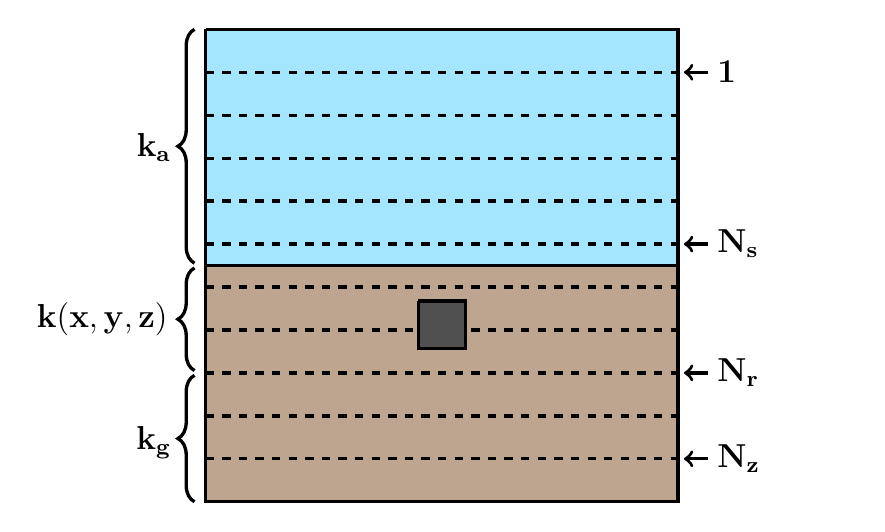
\begin{tikzpicture}[scale=.75]

\def\w{8}; \def\s{\w*.5};

\definecolor{sky}{RGB}{115,215,255};
\definecolor{dirt}{RGB}{155,118,83};
\def\op{.65}

\draw [very thick,fill=sky,fill opacity=\op] (0,0)--(0,-\w)--(\w,-\w)--(\w,0)--(0,0);
\draw [very thick,fill=white] (0,-\s)--(0,-\w)--(\w,-\w)--(\w,-\s)--(0,-\s);
\draw [very thick,fill=dirt,fill opacity=\op] (0,-\s)--(0,-\w)--(\w,-\w)--(\w,-\s)--(0,-\s);

\def\Ny{11};\def\hy{\w/\Ny};
\foreach \j in {1,...,\Ny}{
\draw[very thick, dashed] (0,-\j*\hy)--(\w,-\j*\hy);
}

\def\x{4}; \def\y{-5} \def\r{.4}
\definecolor{mine}{RGB}{80,80,80};
\draw [very thick,fill=mine] (\x-\r,\y+\r)--(\x-\r,\y-\r)--(\x+\r,\y-\r)--(\x+\r,\y+\r)--(\x-\r,\y+\r);

\def\o{.5};
\node[anchor=west] () at (\w+\o,-5*\hy) {\large $\mathbf{\ns}$};
\draw[very thick,->] (\w+\o,-5*\hy)--(\w+\o/5,-5*\hy);
\node[anchor=west] () at (\w+\o,-8*\hy) {\large $\mathbf{\nr}$};
\draw[very thick,->] (\w+\o,-8*\hy)--(\w+\o/5,-8*\hy);

\node[anchor=west] () at (\w+\o,-\hy) {\large $\mathbf{1}$};
\node[anchor=west] () at (\w+\o,-\Ny*\hy+\hy) {\large $\mathbf{\nz}$};
\draw[very thick,->] (\w+\o,-\hy)--(\w+\o/5,-\hy);
\draw[very thick,->] (\w+\o,-\Ny*\hy+\hy)--(\w+\o/5,-\Ny*\hy+\hy);

\node[] () at (-\o*1.75,-\w/4) {\large $\mathbf{k_a}$};
\node[] () at (-\o*3.5,-\w*.625 + .1) {\large $\mathbf{k(x,y,z)}$};
\node[] () at (-\o*1.75,-\w*.875) {\large $\mathbf{k_g}$};

%%Center
\node[anchor=west,text=white] () at (\w+\o,-\w*.625) {\large $\mathbf{k(x,y,z)}$};


\def\nm{8*\hy};
\def\b{.04};
\def\amp{6pt};
\def\ra{4pt};

\draw [very thick, decorate, decoration = {brace,raise=\ra,amplitude=\amp}] (0,-\s+\b) --  (0,0);
\draw [very thick, decorate, decoration = {brace,raise=\ra,amplitude=\amp}] (0,-\nm+\b)--(0,-\s-\b);
\draw [very thick, decorate, decoration = {brace,raise=\ra,amplitude=\amp}] (0,-\w)--(0,-\nm-\b);

\end{tikzpicture}\end{center}
}



\newcommand{\twoDimensionalDomainVariableKyGrid}{
\begin{center}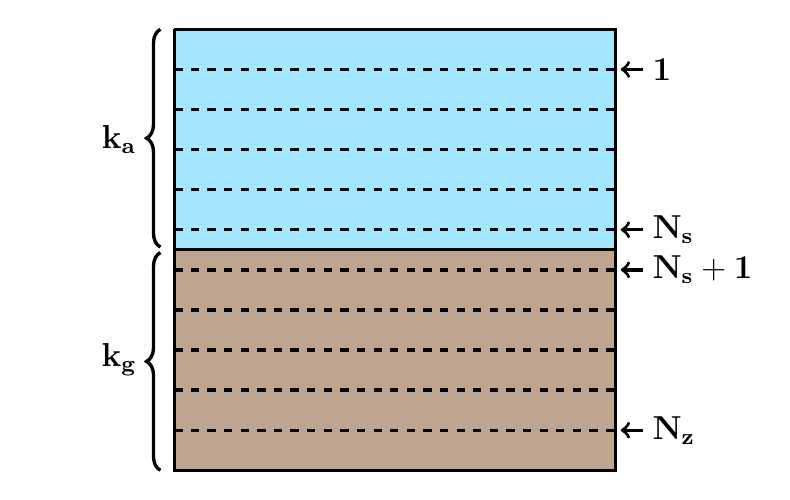
\begin{tikzpicture}[scale=.7]

\def\w{8}; \def\s{\w*.5};

\definecolor{sky}{RGB}{115,215,255};
\definecolor{dirt}{RGB}{155,118,83};
\def\op{.65}
\draw [very thick,fill=sky,fill opacity=\op] (0,0)--(0,-\w)--(\w,-\w)--(\w,0)--(0,0);
\draw [very thick,fill=white] (0,-\s)--(0,-\w)--(\w,-\w)--(\w,-\s)--(0,-\s);
\draw [very thick,fill=dirt,fill opacity=\op] (0,-\s)--(0,-\w)--(\w,-\w)--(\w,-\s)--(0,-\s);

\def\Ny{11};\def\hy{\w/\Ny};
\foreach \j in {1,...,\Ny}{
\draw[very thick, dashed] (0,-\j*\hy)--(\w,-\j*\hy);
}

\def\o{.5};
\node[anchor=west] () at (\w+\o,-5*\hy) {\large $\mathbf{\ns}$};
\node[anchor=west] () at (\w+\o,-6*\hy) {\large $\mathbf{\ns + 1}$};
\node[anchor=east,text=white] () at (-\o,-6*\hy) {\large $\mathbf{\ns + 1}$};
\draw[very thick,->] (\w+\o,-5*\hy)--(\w+\o/5,-5*\hy);
\draw[very thick,->] (\w+\o,-6*\hy)--(\w+\o/5,-6*\hy);

\node[anchor=west] () at (\w+\o,-\hy) {\large $\mathbf{1}$};
\node[anchor=west] () at (\w+\o,-\Ny*\hy+\hy) {\large $\mathbf{\nz}$};
\draw[very thick,->] (\w+\o,-\hy)--(\w+\o/5,-\hy);
\draw[very thick,->] (\w+\o,-\Ny*\hy+\hy)--(\w+\o/5,-\Ny*\hy+\hy);
%\draw[very thick,->] (-\o*1.65,-\hy-\o)--(-\o*1.65,-\Ny*\hy+\hy+\o);

\node[] () at (-\o*2,-\w/4) {\large $\mathbf{k_a}$};
\node[] () at (-\o*2,-\w*.75) {\large $\mathbf{k_g}$};

\draw [very thick, decorate, decoration = {brace,raise=5pt,amplitude=5pt}] (0,-\s+.05) --  (0,0);
\draw [very thick, decorate, decoration = {brace,raise=5pt,amplitude=5pt}] (0,-\w)--(0,-\s-.05);

\end{tikzpicture}\end{center}
}



\newcommand{\twoDimensionalDomainVariableKyGridSolver}{
\begin{center}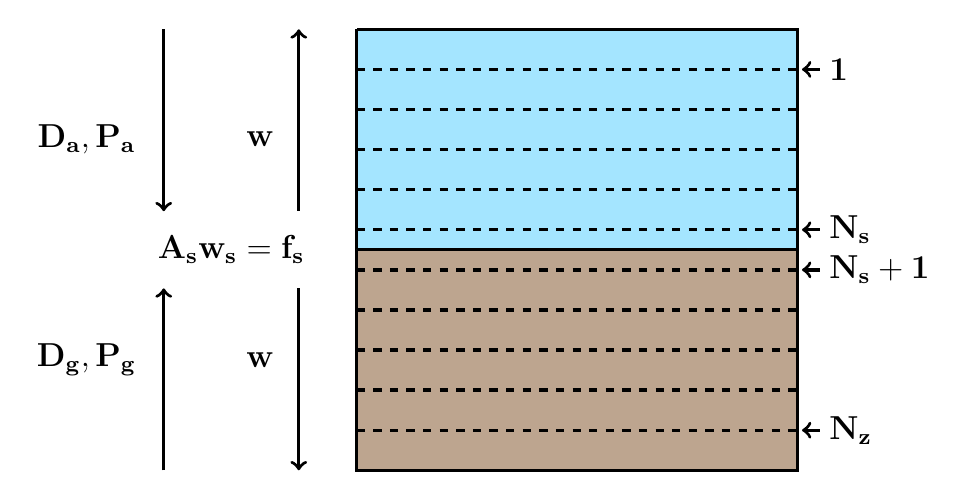
\begin{tikzpicture}[scale=.7]

\def\w{8}; \def\s{\w*.5};

\definecolor{sky}{RGB}{115,215,255};
\definecolor{dirt}{RGB}{155,118,83};
\def\op{.65}
\draw [very thick,fill=sky,fill opacity=\op] (0,0)--(0,-\w)--(\w,-\w)--(\w,0)--(0,0);
\draw [very thick,fill=white] (0,-\s)--(0,-\w)--(\w,-\w)--(\w,-\s)--(0,-\s);
\draw [very thick,fill=dirt,fill opacity=\op] (0,-\s)--(0,-\w)--(\w,-\w)--(\w,-\s)--(0,-\s);

\def\Ny{11};\def\hy{\w/\Ny};
\foreach \j in {1,...,\Ny}{
\draw[very thick, dashed] (0,-\j*\hy)--(\w,-\j*\hy);
}

\def\o{.4};
\node[anchor=west] () at (\w+\o,-5*\hy) {\large $\mathbf{\ns}$};
\node[anchor=west] () at (\w+\o,-6*\hy) {\large $\mathbf{\ns + 1}$};
\node[anchor=east,text=white] () at (-\o,-6*\hy) {\large $\mathbf{\ns + 1}$};
\draw[very thick,->] (\w+\o,-5*\hy)--(\w+\o/5,-5*\hy);
\draw[very thick,->] (\w+\o,-6*\hy)--(\w+\o/5,-6*\hy);

\node[anchor=west] () at (\w+\o,-\hy) {\large $\mathbf{1}$};
\node[anchor=west] () at (\w+\o,-\Ny*\hy+\hy) {\large $\mathbf{\nz}$};
\draw[very thick,->] (\w+\o,-\hy)--(\w+\o/5,-\hy);
\draw[very thick,->] (\w+\o,-\Ny*\hy+\hy)--(\w+\o/5,-\Ny*\hy+\hy);
%\draw[very thick,->] (-\o*1.65,-\hy-\o)--(-\o*1.65,-\Ny*\hy+\hy+\o);

%\node[] () at (-\o*2,-\w/4) { ${k_a}$};
%\node[] () at (-\o*2,-\w*.75) { ${k_g}$};
%
%\draw [thick, decorate, decoration = {brace,raise=5pt,amplitude=5pt}] (0,-\s+.05) --  (0,0);
%\draw [thick, decorate, decoration = {brace,raise=5pt,amplitude=5pt}] (0,-\w)--(0,-\s-.05);

\def\ms{.7};
\def\o{.7};
\node[] () at (-\o*7,-\w/4) {\large $\mathbf{D_a},\mathbf{P_a}$};
\draw[very thick,->] (-\o*5,0)--(-\o*5,-\s+\ms);

\node[] () at (-\o*7,-3*\w/4) {\large $\mathbf{D_g},\mathbf{P_g}$};
\draw[very thick,->] (-\o*5,-\w)--(-\o*5,-\s-\ms);


\node[] () at (-\o*2.5,-\w/4) {\large $\vec{w}$};
\draw[very thick,<-] (-\o*1.5,0)--(-\o*1.5,-\s+\ms);

\node[] () at (-\o*2.5,-3*\w/4) {\large $\vec{w}$};
\draw[very thick,<-] (-\o*1.5,-\w)--(-\o*1.5,-\s-\ms);

\node[] () at (-\o*3.25,-\w/2) {\large $\mathbf{A_s\vec{w}_s = \vec{f}_s}$};


\end{tikzpicture}\end{center}}

 
\begin{document}
 
\frame{\titlepage}


\begin{frame}{Introduction}
\begin{itemize}
\item Novel direct parallel partial FFT-type algorithm for the numerical solutions of the two- and three-dimensional Helmholtz equations.\\[1em]
\item Governing equations are discretized by high-order compact finite-difference schemes.\\[1em]
%\item Parallel direct approaches are a better alternative to iterative methods in this situation.\\[1em]
\item Accuracy and scalability of the direct parallel method are investigated on scattering problems with realistic ranges of parameters for air, soil and mine-like targets.\\[1em]
\end{itemize}
\end{frame}


%\begin{frame}{Introduction}
%In this presentation, a novel direct parallel partial FFT-type algorithm for the numerical solutions of the two- and three-dimensional Helmholtz equations is given. The governing equations are discretized by high-order compact finite-difference or finite-element methods. The resulting discretized system is indefinite, making the convergence of most iterative methods deteriorate as frequency increases. In this situation, the parallel direct approaches are a better alternative. The complexity and scalability of the direct parallel method are investigated on scattering problems with realistic ranges of parameters for air, soil and mine-like targets.
%\end{frame}


\begin{frame}{Outline}
\begin{itemize}
%\item General Concept\\[1em]
\item Model Problem\\[1em]
\item Research Chronology\\[1em]
\item Discretization\\[1em]
\item Direct Parallel FFT Solver\\[1em]
\item Direct Parallel Eigenvalue Solver\\[1em]
\item Direct Parallel Partial FFT Solver\\[1em]
\item Numerical Results\\[1em]
\end{itemize}
\end{frame}





%\begin{frame}{General Concept}
%	include explanation of discretization, (pde to matrix equation)
%	Example of how matrix equations grow and how Gaussian elimination grows
%	Explain resolution/ solution accuracy in scientific application
%	Higher Frequency needed for detecting small mines
%\end{frame}



%////////////////////////////////////////////////////////////////////////
%///////////////////////////////// HELM /////////////////////////////////
%////////////////////////////////////////////////////////////////////////


\begin{frame}{Model Problem}
The two- and three-dimensional \helm equations on a rectangular domains. That is
\begin{equation}
\Delta u(\vec{x})+k^2(\vec{x})u(\vec{x})=f(\vec{x})\ \  \text{in}  \ \Omega.\nonumber%\label{eqn:general_Helmholtz}
\end{equation}
The domain is defined as $\Omega =\left\{ \vec{x}=(x,y,z) \in \R^3 \mid x_l \le x\le x_u, \, y_l \le y\le y_u, \, z_l \le z\le z_u\right\}$ where $ x_l < x_u$, $ y_l < y_u$ and $z_l<z_u$. The function $k$ is complex valued. Dirichlet and \somm boundary conditions are considered.
\end{frame}


\begin{frame}{Research Chronology}
\textbf{Construction of Higher-Order Compact Schemes:}\\
Lele (1992),\\
Nabadi, Siddiqui and Dargahi (2007),\\
Sutmann (2007),\\
Turkel, D. Gordon, R. Gordon and Tsynkov (2013).\\[1em]
\textbf{Second-Order FD and FEM + GMRES + FFT}\\
Elman and O'Leary (1998),\\
Gryazin, Klibanov and Lucas (2000).\\[1em]
\end{frame}


\begin{frame}{Research Chronology}
\textbf{Parallel Compact Higher-Order Schemes+GMRES+FFT:}\\
Gryazin, Lee and Gonzales (2019),\\
Gonzales, Gryazin and Lee (2021).\\[1em]
\textbf{Partial FFT Solver for Compact Schemes:}\\
Toivanen and Wolfmayr (2020).\\[1em]
\textbf{Parallel Partial FFT Solver for High-Order Compact Schemes:}\\
Gonzales and Gryazin (2022).\\[1em]
\end{frame}


%%%History 
%%%Parallel omp compact schemes fft-type alg
%%%-our paper 2021
%%%-dirrect pfft solver + compact schemes 2022 
%%%
%%%High order compact schemes parallel 
%%%
%%%2nd order finite diff schemes+finite element schemes
%%%-Elmond and lear (last two in dr g)
%%%
%%%Construction of compact schemes
%%%
%%%High order comp schemes + openmp
%%%2019
%%%High order comp schemes + hybrid par paper
%%%Pfft solver for high + compact schemes
%%%-toiv. (Explain toil for constant for 2nd and 4th)
%%%-our SPIE  (we extend to layered with interface with 2nd fourth and sixth)


%////////////////////////////////////////////////////////////////////////
%//////////////////////////////// SCHEME ////////////////////////////////
%////////////////////////////////////////////////////////////////////////

\begin{frame}{Second-Order Compact Scheme}

Consider the following notation for the first and second central differences at the $(i, j, l)$-th grid point
\begin{align}
\fdiffo{x}u_\ind &=\fdiff[l]{u}{i}{j}{x}, \eqntab \sdiffo{x}u_\ind=\sdiff[l]{u}{i}{j}{x}\nonumber
\end{align}
where $u_{i,j,l}=u(x_i,y_j,z_l)$. Then the standard second-order scheme is given by
\begin{align*}
&\frac{1}{h_x^2}u_{i-1,j,l} + \frac{1}{h_y^2}u_{i,j-1,l} + \frac{1}{h_z^2}u_{i,j,l-1} +\left(k_{i,j,l}^2 - \frac{2}{h_x^2}-\frac{2}{h_y^2}-\frac{2}{h_z^2}\right)u_{i,j,l} \\[1em]
&\eqntab +\frac{1}{h_x^2}u_{i+1,j,l}+ \frac{1}{h_y^2}u_{i,j+1,l} + \frac{1}{h_z^2}u_{i,j,l+1} = f_{i,j,l}.
\end{align*}
\end{frame}

\begin{frame}{Fourth-Order Compact Scheme}
\begin{align*}
& \l(1+h_x^2\frac{\sdiffo{x}}{12}+h_y^2\frac{\sdiffo{y}}{12}+h_z^2\frac{\sdiffo{z}}{12}\r)k_{i,j,l}^2u_{i,j,l}\\[1em]
%
&+ \l(\sdiffo{x}+h_y^2\frac{\sdiffo{x}\sdiffo{y}}{12}+h_z^2\frac{\sdiffo{x}\sdiffo{z}}{12}\right)u_{i,j,l} + \left(\sdiffo{y}+h_x^2\frac{\sdiffo{x}\sdiffo{y}}{12}+h_z^2\frac{\sdiffo{y}\sdiffo{z}}{12}\r)u_{i,j,l} \\[1em]
%
&+ \l(\sdiffo{z}+h_x^2\frac{\sdiffo{x}\sdiffo{z}}{12}+h_y^2\frac{\sdiffo{y}\sdiffo{z}}{12}\r)u_{i,j,l}  = \l(1+h_x^2\frac{\sdiffo{x}}{12}+h_y^2\frac{\sdiffo{y}}{12}+h_z^2\frac{\sdiffo{z}}{12}\r)f_{i,j,l}
\end{align*}
\textbf{Lele (1992)}
%\textbf{Gonzales, Gryazin and Lee (2021)}
\end{frame}


\begin{frame}{Sixth-Order Notation}
\vspace{-1cm}
\begin{align*}
\laplaceh u_\ind &= \l(\sdiffo{x} + \sdiffo{y} + \sdiffo{z}\r)u_\ind \\[1em]
L_hu_\ind &= (\laplaceh + k^2_\ind) u_\ind\\[1em]
\gradh u_\ind &= \l(\fdiffo{x}\,,\,\fdiffo{y} \,,\,\fdiffo{z}\r)u_\ind \\[1em]
%
\gradp u_\ind &= \l(\fdiffo{x}\sdiffo{y} \,,\,\sdiffo{x}\fdiffo{y} \,,\,\sdiffo{x}\fdiffo{z}\r)u_\ind + \l(\fdiffo{x}\sdiffo{z}\,,\, \fdiffo{y}\sdiffo{z} \,,\, \sdiffo{y}\fdiffo{z} \r)u_\ind \\[1em]
%
%\laplaceh u_\ind &= \l(\sdiffo{x} + \sdiffo{y} + \sdiffo{z}\r)u_\ind \\[1em]
%
\grad^4 u&= \l(\pd{x,x,x,x}+\pd{y,y,y,y}+\pd{z,z,z,z}\r)u
\end{align*}
%\textbf{Turkel, D. Gordon, R. Gordon, and Tsynkov (2013)}
%\textbf{Gonzales, Gryazin and Lee (2021)}
\end{frame}


\begin{frame}{Sixth-Order Compact Scheme}
\vspace{-.7cm}
\begin{multline*}
L_hu_\ind + \frac{h^2}{6}\l(\sdiffo{x}\sdiffo{y} + \sdiffo{x}\sdiffo{z} + \sdiffo{y}\sdiffo{z}\r)u_\ind +\frac{h^2}{20}  \l( \laplace k_\ind^2 - k_\ind^4 \r)u_\ind   \\[1em]
+ \frac{h^2}{10} \grad k_\ind^2 \cdot \gradh u_\ind + \frac{h^4}{60}\grad k_\ind^2 \cdot\l( \gradp u_\ind + \gradh\l(k^2u\r)_\ind  \r)  \\[1em]
+ \frac{h^4}{30}\sdiffo{x}\sdiffo{y}\sdiffo{z}u_\ind +\dfrac{h^2}{30}   \laplaceh\left(k^2u\r)_\ind + \frac{h^4}{90}\l(\sdiffo{x}\sdiffo{y} + \sdiffo{x}\sdiffo{z} + \sdiffo{y}\sdiffo{z}\r)\l(k^2u\r)_\ind  \\[1em]
=\l(1- \frac{h^2}{20} k_\ind^2\r)f_\ind + \frac{h^2}{12}\laplace f_\ind + \frac{h^4}{60}\grad k_\ind^2 \cdot \grad f_\ind + \frac{h^4}{360} \grad^4 f_\ind \\[1em]
+ \frac{h^4}{90}\l(\pd{x,x,y,y}+ \pd{x,x,z,z} + \pd{y,y,z,z}\r)f_\ind % \eqntab \cite{turkel,parallel_paper}
\end{multline*}
\textbf{Turkel, D. Gordon, R. Gordon, and Tsynkov (2013)}
\end{frame}





%////////////////////////////////////////////////////////////////////////
%///////////////////////////////// BND /////////////////////////////////
%////////////////////////////////////////////////////////////////////////



\begin{frame}{\Somm Boundary Conditions}
The Sommerfeld radiation conditions are
\[\lim\limits_{r\rightarrow\infty} r^{(d-1)/2}\l(\frac{\partial}{\partial r}u(\vec{x}) -ik(\vec{x}) u(\vec{x}) \r) = 0\]
with $d=2$ or $d=3$ for two- and three-dimensions respectively. Truncating the unbounded domain to a finite domain at the boundary under consideration provides the approximation. That is
\[\grad u(\vec{x})\cdot\vec{n} -ik(\vec{x})u(\vec{x}) = 0 %\numbereqn\label{bnd:somm}
\]
for $\vec{x}\in\partial \Omega$ where $\vec{n}$ is the outward normal vector of the boundary. 

%\textbf{Gryazin, Klibanov and Lucas (2000)}
\end{frame}


\begin{frame}{\Somm Boundary Conditions Approximation}
The ninth-order approximation for the \somm boundary conditions on the $x$ boundaries are
\begin{align*}
u_{\iota\pm1,j,l} & = u_{\iota\mp1,j,l} + 2i\hx k_{j,l}\l(1 - \frac{h_x^2k^2_{j,l}}{3!} +  \frac{h_x^4k^4_{j,l}}{5!} -  \frac{h_x^6k_{j,l}^6}{7!} \r)u_{\iota,j,l}\\[1em]
 %
&= u_{\iota\mp1,j,l} + \alpha_{x,j,l}u_{\iota, j, l}
%
% u_{\iota-1,j,l}  & = u_{\iota+1,j,l} + 2i\hx k_{j,l}\l(1 - \frac{h_x^2k^2_{j,l}}{3!} +  \frac{h_x^4k^4_{j,l}}{5!} -  \frac{h_x^6k_{j,l}^6}{7!}\r)u_{\iota,j,l} +\bigo{\hx^7}\\[1em]
 %
%u_{\iota-1,j,l}&=\beta_{x}u_{\iota+1,j,l} + \alpha_{x,j,l}u_{\iota, j, l}  +\bigo{h_x^7}
\end{align*}
where $\alpha_{x,j,l} = 2i\hx k_{j,l}\l(1 - {h_x^2k^2_{j,l}}/{3!} +  {h_x^4k^4_{j,l}}/{5!} -  {h_x^6k_{j,l}^6}/{7!} \r)$. The coefficients $\alpha_{y,\iota,l}$ and $\alpha_{z,\iota,j}$ are found in the same way. %The pattern in the stencil breaks down when including these conditions on all boundaries and is therefore unsuitable for the FFT Solver.
\end{frame}




%////////////////////////////////////////////////////////////////////////
%///////////////////////////////// FFT /////////////////////////////////
%////////////////////////////////////////////////////////////////////////




\begin{frame}{Parallel FFT Solver for Compact Schemes}

\begin{itemize}
\item Assumptions for the parallel FFT solver
\begin{itemize}
\item \somm conditions on the top and bottom boundaries with respect to the vertical direction
\item Dirichlet conditions on the other boundaries
\item The coefficient $k$ varies only vertically, i.e. $k(\vec{x}) = k(z)$\\
\end{itemize}

\item These conditions produce a stencil pattern that ensures the eigenvalues and eigenvectors of the linear system $A\vec{u}=\vec{f}$ can be represented in terms of real valued functions, i.e. sines and cosines.\\

\item Allows the use of FFT for the diagonalization of the system.\\

\item Solver steps
\begin{itemize}
\item Forward transform (diagonalization)
\item Solution
\item Reverse transform
\end{itemize}
\end{itemize}


%Here it is assumed that \somm boundary conditions are only considered on the top and bottom of the domain with respect to the vertical direction and Dirichlet conditions on the remaining boundaries. Also, $k$ is assumed to vary only vertically, i.e. $k(\vec{x}) = k(z)$.
%
%\begin{itemize}
%\item more on general solver for compact schemes with conditions on stencil
%\item we can actually use this solver for finite element app
%\end{itemize}
%
%we have cond. on our coef which ensure our e-val can be rep in terms of real val funct cosines so we can use FFT for the diagonalization of the system and then solution

%Put convection diffusion and support us IN BOLD
%
%Couple more slides on general solver for compact schemes with conditions on stencil and put another slide on convection diffusion we can actually use this solver for finite element app. (In paper) or can even solve different pde’s like cone-diff for atmospheric flows and put slide from siam. Talk about how limit to Dirichlet Neumann and periodic BC then we need more robust solver for ABC 

%Couple more slides on general solver for compact schemes with conditions on stencil and put another slide on convection diffusion we can actually use this solver for finite element app. 

\end{frame}



%\begin{frame}
%The compact schemes can be expressed at every grid point $(\ind)$ as
%\begin{align*}
%\sum\limits_{\nu=l-1}^{l+1} &\l(d_\nu \l[u_{i-1,j-1,\nu} + u_{i-1,j+1,\nu} + u_{i+1,j-1,\nu} + u_{i+1,j+1,\nu}\r]\r.\\[1em]
%%
%&+b_\nu \l.\l[u_{i-1,j,\nu} + u_{i+1,j,\nu}\r] + c_\nu \l[u_{i,j-1,\nu} + u_{i,j+1,\nu}\r]  + a_\nu u_{i,j,\nu}\r)\\[1em]
%& = f_\ind
%\end{align*}
%corresponding to the $\l(i+(j-1)\cdot N_x + (l-1)\cdot N_x\cdot N_y\r) - th$ row in the resulting linear system 
%\[A\vec{u} = \vec{f}.\]
%\end{frame}




\begin{frame}{27 Point Stencil Symmetry for Parallel FFT Solver}
\begin{center}
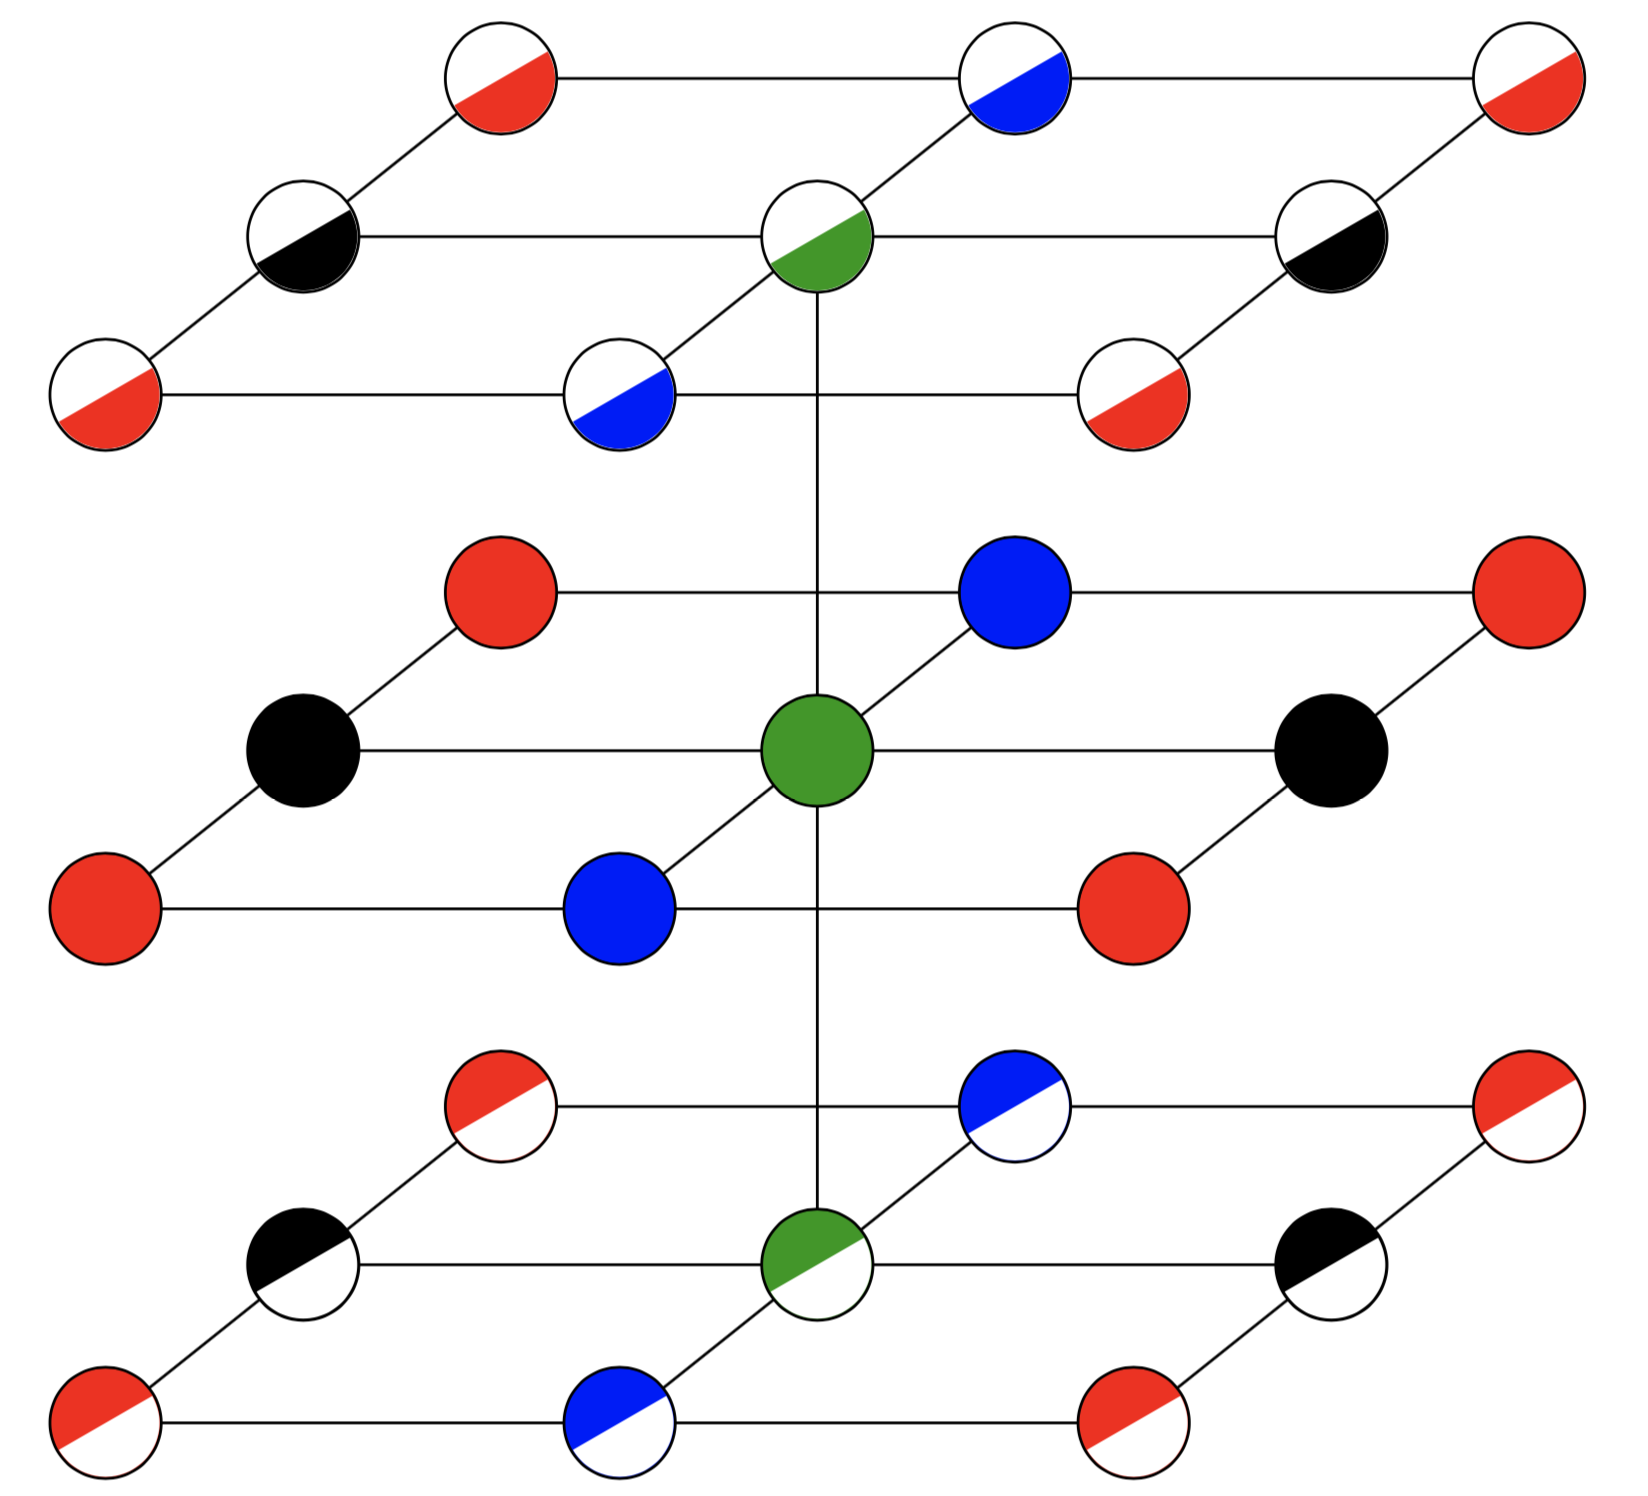
\includegraphics[scale=.2]{images/color_stencil}
\end{center}
\textbf{Gonzales, Gryazin and Lee (2021)}
\end{frame}




\begin{frame}{Parallelization}
\begin{center}
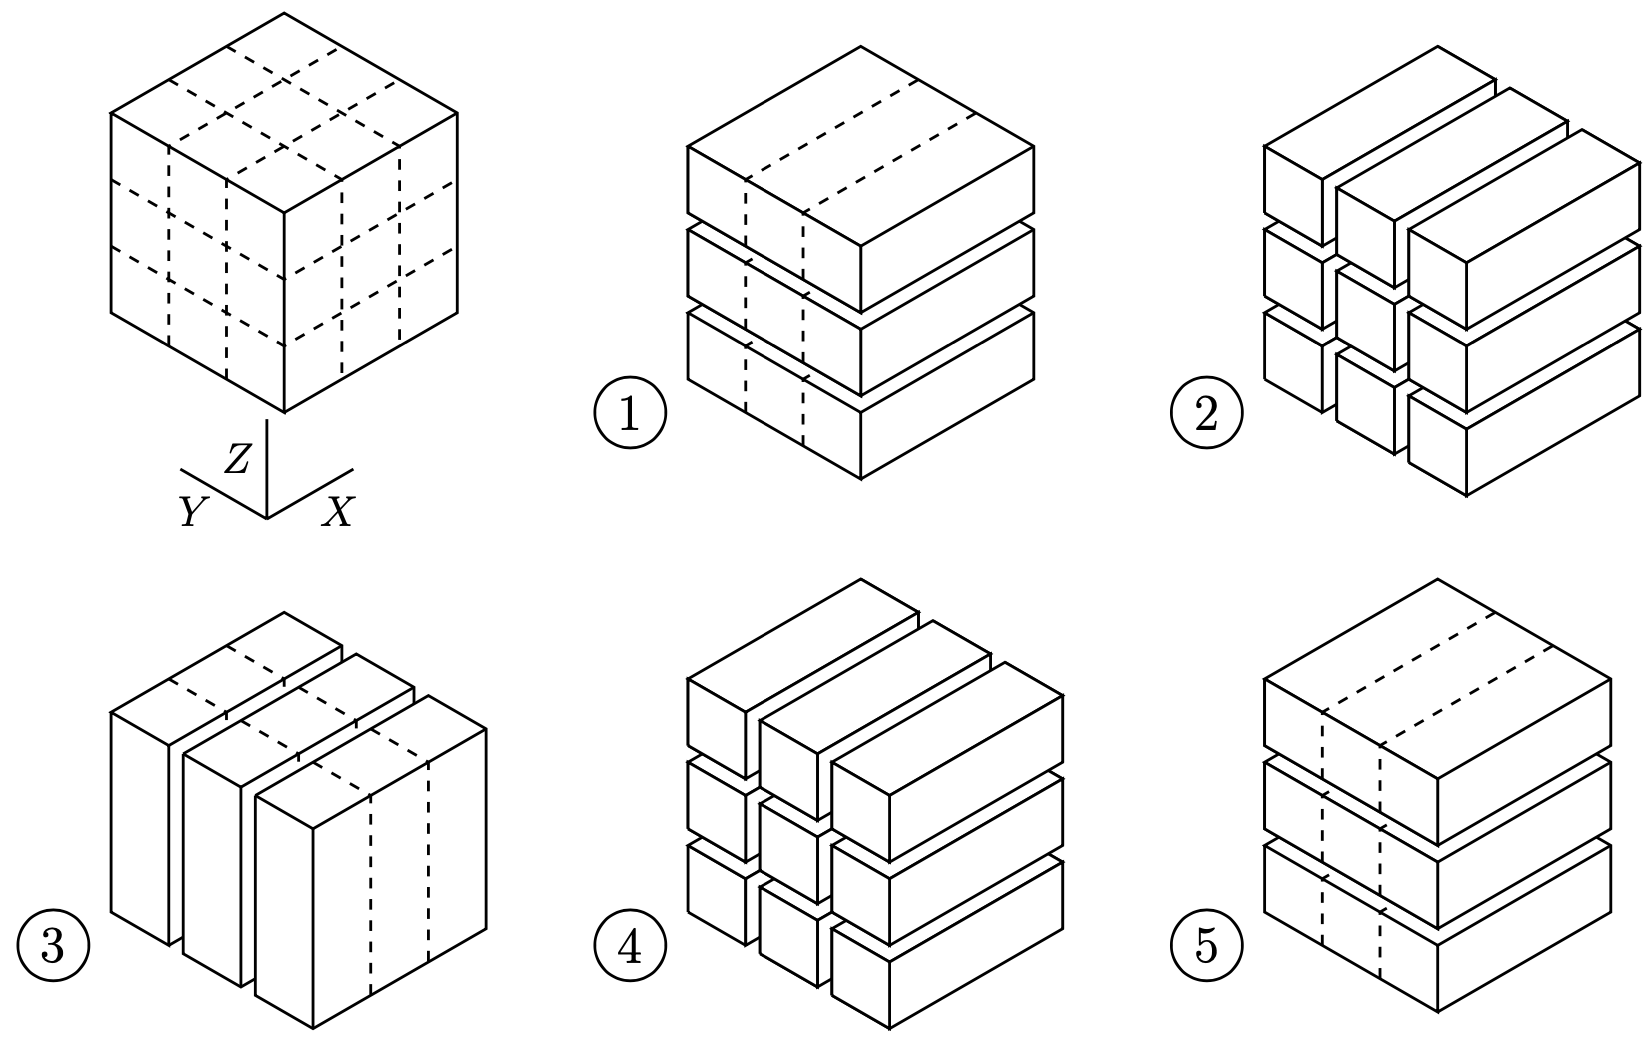
\includegraphics[scale=.37]{images/mpi_image}
\end{center}
\end{frame}


\begin{frame}{Parallel FFT Solver}
\begin{algorithm}[H]
\caption{Parallel FFT Solver}\label{alg:general_parallel_fft}
\begin{algorithmic}[1]
\STATE Find array indexes that evenly split work, i.e. $start_y$, $end_y$, $start_z$, and $end_z$
\FOR{$l=start_z\dots end_z$}
\STATE 2D forward DST in $x-$ and $y-$ directions via \FFT
\ENDFOR
\STATE Transfer data via MPI if in a distributed memory environment
\FOR{$j=start_y\dots end_y;\,i=1\dots \nx$}
\STATE Solve the tridiagonal system using LU decomposition
\ENDFOR
\STATE Transfer data via MPI if in a distributed memory environment
\FOR{$l=start_z\dots end_z$}
\STATE 2D inverse DST in $x-$ and $y-$ directions via \FFT
\ENDFOR
\end{algorithmic}
\end{algorithm}
\end{frame}


\begin{frame}{Parallel FFT Solver Versatility}
\begin{itemize}
\item The parallel FFT solver can solve different PDEs, e.g. the Convection-Diffusion equation. \\[1em]

\item This solver is limited to Dirichlet, Neumann and periodic boundary conditions. \\[1em]

\item A more generalized solver for the case of absorbing boundary conditions, i.e. \somm, is required.

\end{itemize}


%\begin{itemize}
%\item can even solve different pde’s like cone-diff for atmospheric flows
%\item stuff from SIAM talk
%\item transition to PFFT (Talk about how limit to Dirichlet Neumann and periodic BC then we need more robust solver for ABC )
%\end{itemize}

%\textbf{Gonzales and Gryazin (2022)}
\end{frame}






%////////////////////////////////////////////////////////////////////////
%///////////////////////////////// EIG /////////////////////////////////
%////////////////////////////////////////////////////////////////////////



%///////////////////////////////// PRE /////////////////////////////////



%\begin{frame}{Eigenvalue Solver Notation}
%The system with \somm conditions on all boundaries and $k$ varying as in the domain with an air, soil and subsurface inclusion requires another solver. Consider the following notation. \\[1em]
%
%Define $\ns$ as the vertical index that is the last to contain the air coefficient $k_a$ and $\nr$ as the first vertical index after the inclusion. Let the matrices $A_a$, $B_a$, $A_g$, $B_g$, $C_{l}$, $A_{l}$, and $B_{l}\in\C^{\nx\cdot\ny\times\nx\cdot\ny}$ be generated from the general 27-point stencil.  \\[1em]
%
%To partially diagonalize the resulting system consider
%\vspace{-2mm}
%\begin{align*}
%\vec{w}_l& = S^{-1}\vec{u}_l \text{ and } \bar{\vec{f}}_l = S^{-1}B_a^{-1}\vec{f}_l \eqntab\text{ for }l=1,\dots,N_s\\
%%
%\vec{w}_l& = R^{-1}\vec{u}_l \text{ and } \bar{\vec{f}}_l = R^{-1}B_g^{-1}\vec{f}_l \eqntab\text{ for }l=\nr,\dots,\nz.
%\end{align*}
%\end{frame}

\begin{frame}{Domain with Air and Soil Interface}
\twoDimensionalDomainVariableKyGrid
\end{frame}

%\begin{frame}{Parallel Eigenvalue Solver Notation}
%The system with \somm conditions on all boundaries requires another solver. Consider the following notation. \\[1em]
%
%Define $\ns$ as the vertical index that is the last to contain the constant air coefficient $k_a$. The remaining layers contain the constant soil coefficient $k_g$. Let the matrices $A_a$, $B_a$, $A_g$, and $B_g\in\C^{\nx\cdot\ny\times\nx\cdot\ny}$ be generated from the general 27-point stencil.  \\[1em]
%
%To partially diagonalize the resulting system consider
%\vspace{-2mm}
%\begin{align*}
%\vec{w}_l& = S^{-1}\vec{u}_l \text{ and } \bar{\vec{f}}_l = S^{-1}B_a^{-1}\vec{f}_l \eqntab\text{ for }l=1,\dots,N_s\\
%%
%\vec{w}_l& = R^{-1}\vec{u}_l \text{ and } \bar{\vec{f}}_l = R^{-1}B_g^{-1}\vec{f}_l \eqntab\text{ for }l=\ns+1,\dots,\nz.
%\end{align*}
%\end{frame}

\begin{frame}{Parallel Eigenvalue Solver Notation}
\begin{itemize}
\item \somm conditions on all boundaries.\\[1em]
\item Define $\ns$ as the vertical index that is the last to contain the constant air coefficient $k_a$.\\[1em]
\item Matrices $A_a$, $B_a$, $A_g$, and $B_g\in\C^{\nx\cdot\ny\times\nx\cdot\ny}$ are generated from the FFT solver 27-point stencil.\\[1em]
%\item $S$ and $R$ are the matrices of eigenvectors 
\item Consider the generalized eigenvalues $A_a S = B_a S\Lambda_a$  and $A_g R = B_g R\Lambda_g$.\\[1em]
\item $\vec{w}_l = S^{-1}\vec{u}_l \text{ and } \bar{\vec{f}}_l = S^{-1}B_a^{-1}\vec{f}_l \eqntab\text{ for }l=1,\dots,N_s$\\[1em]
\item $\vec{w}_l = R^{-1}\vec{u}_l \text{ and } \bar{\vec{f}}_l = R^{-1}B_g^{-1}\vec{f}_l \eqntab\text{ for }l=\ns+1,\dots,\nz$
\end{itemize}
%The system with \somm conditions on all boundaries requires another solver. Consider the following notation. \\[1em]
%
%Define $\ns$ as the vertical index that is the last to contain the constant air coefficient $k_a$. The remaining layers contain the constant soil coefficient $k_g$. Let the matrices $A_a$, $B_a$, $A_g$, and $B_g\in\C^{\nx\cdot\ny\times\nx\cdot\ny}$ be generated from the general 27-point stencil.  \\[1em]
%
%To partially diagonalize the resulting system consider
%\vspace{-2mm}
%\begin{align*}
%\vec{w}_l& = S^{-1}\vec{u}_l \text{ and } \bar{\vec{f}}_l = S^{-1}B_a^{-1}\vec{f}_l \eqntab\text{ for }l=1,\dots,N_s\\
%%
%\vec{w}_l& = R^{-1}\vec{u}_l \text{ and } \bar{\vec{f}}_l = R^{-1}B_g^{-1}\vec{f}_l \eqntab\text{ for }l=\ns+1,\dots,\nz.
%\end{align*}
\end{frame}




\begin{frame}
The partially diagonalized system is given by
\begin{align*}
\l(\Lambda_a+\alpha_aI \r)\vec{w}_1 + \l(1+\beta_a\r)\vec{w}_2 &= \hat{\vec{f}}_1 \\
%
\vec{w}_{l-1}+\Lambda_a\vec{w}_l+\vec{w}_{l+1}&= \hat{\vec{f}}_l\eqntab \text{ for }l=2,\dots, \ns-1 \\
%
\vec{w}_{\ns-1}+\Lambda_a\vec{w}_\ns+M\vec{w}_{\ns+1}&= \hat{\vec{f}}_\ns \\
%
M^{-1}\vec{w}_{\ns}+\Lambda_g\vec{w}_{\ns+1}+\vec{w}_{\ns+2}&= \hat{\vec{f}}_{\ns+1} \\
%
\vec{w}_{l-1}+\Lambda_g\vec{w}_l+\vec{w}_{l+1}&= \hat{\vec{f}}_l\eqntab \text{ for }l=\ns+2,\dots, \nz-1 \\
%
\l(1+\beta_g\r)\vec{w}_{\nz-1} + \l(\Lambda_g+\alpha_g I\r)\vec{w}_\nz &= \hat{\vec{f}}_\nz
\end{align*}
where $M=S^{-1}B_a^{-1}B_gR$ and $\alpha_a$, $\alpha_g$, $\beta_a$ and $\beta_g$ are coefficients from the approximation of the \somm boundary conditions.
\end{frame}

\begin{frame}
To solve this transformed tridiagonal system assume that
\begin{align*}
\vec{w}_l &= D_{a,l}\vec{w}_{l+1} + P_{a,l}\eqntab \text{ for }l=1,\dots, \ns-1
\end{align*}
It follows that
\begin{align*}
D_{a,1} &= - 2\l( \Lambda_a + \alpha_aI\r)^{-1} \text{ and } P_{a,1}=\l( \Lambda_a + \alpha_aI\r)^{-1}\bar{\vec{f}}_1\\[1em]
%
D_{a,l} &= -\l(\Lambda_a\ + D_{a,l-1}\r)^{-1} \text{ and } P_{a,l} = \l(\Lambda_a\ + D_{a,l-1}\r)^{-1}\l(\bar{\vec{f}}_l - P_{a,l-1}\r)
\end{align*}
for $l=1,\dots, \ns-1$.
\end{frame}


\begin{frame}
In the opposite direction, consider
\begin{align*}
\vec{w}_{l} &= D_{g,l}\vec{w}_{l-1} + P_{g,l}\eqntab \text{ for }l=\nz,\dots, \ns+2.
\end{align*}
It follows that
\begin{align*}
D_{g,\nz} &= -2\l(\Lambda_g+\alpha_gI\r)^{-1} \text{ and } P_{g,\nz} = \l(\Lambda_g+\alpha_gI\r)^{-1}\bar{\vec{f}}_\nz \\[1em]
%
D_{g,l}&=-\l(\Lambda_g + D_{g,l+1}\r)^{-1} \text{ and } P_{g,l}=\l(\Lambda_g + D_{g,l+1}\r)^{-1}\l(\bar{\vec{f}}_l - P_{g,l+1}\r)
\end{align*}
for $l=\nz,\dots, \ns+2$.
\end{frame}

\begin{frame}
The layers remaining are 
\begin{align*}
\vec{w}_{\ns-1}+\Lambda_a\vec{w}_\ns+M\vec{w}_{\ns+1}&= \hat{\vec{f}}_\ns \\
%
M\vec{w}_{\ns}+\Lambda_g\vec{w}_{\ns+1}+\vec{w}_{\ns+2}&= \hat{\vec{f}}_{\ns+1}.
\end{align*}
These layers form the two by two block system $A_s\vec{w}_s=\vec{f}_s$ solved by LU factorization. The remaining transformed solution is computed by 
\begin{align*}
\vec{w}_l &= D_{a,l}\vec{w}_{l+1} + P_{a,l}\eqntab\text{ for }l=\ns-1,\dots,1\\
\vec{w}_l &= D_{g,l}\vec{w}_{l-1} + P_{g,l}\eqntab\text{ for }l=\ns+2,\dots,\nz.
\end{align*}
\end{frame}

\begin{frame}{Basic Idea}
\twoDimensionalDomainVariableKyGridSolver

\textbf{Gonzales and Gryazin (2022)}
\end{frame}


\newcommand{\myfor}[2]{\STATE #2 \tab \textbf{for } {#1} }
\newcommand{\algorithmSpacing}{1.35} %temporary, look into this

\begin{frame}{Parallel Generalized Eigenvalue Solver}
\begin{algorithm}[H]
\caption{Parallel Generalized Eigenvalue Solver}\label{alg:general_eigenvalue_solver}
\begin{spacing}{\algorithmSpacing}
\begin{algorithmic}[1]
\STATE Preliminarily $S$, $S^{-1}$,  $\Lambda_a$, $R$, $R^{-1}$, $\Lambda_g$, $D_a$, $D_g$, and the LU of $A_s$.
\myfor{$l=1,\dots, \ns$}{$\hat{\vec{f}}_l = S^{-1}B_a^{-1}\vec{f}_l$}
\myfor{$l=\ns+1,\dots, \nz$}{$\hat{\vec{f}}_l = R^{-1}B_g^{-1}\vec{f}_l$}
\STATE Compute $P_a$ and $P_g$
\STATE Solve $A_s\vec{w}_s = \vec{f}_s$ via LU decomposition.
\myfor{$l=\ns-1,\dots, 1$}{$\vec{w}_l = D_{a,l}\vec{w}_{l+1} + P_{a,l}$}
\myfor{$l=\ns+2,\dots, \nz$}{$\vec{w}_l = D_{g,l}\vec{w}_{l-1} + P_{g,l}$}
\myfor{$l=1,\dots, \ns$}{$\vec{u}_l = S\vec{w}_1$}
\myfor{$l=\ns+1,\dots, \nz$}{$\vec{u}_l = R\vec{w}_l$}
\end{algorithmic}
\end{spacing}
\end{algorithm}
\end{frame}

%///////////////////////////////// INC /////////////////////////////////


\begin{frame}{Air and Soil Domain with Subsurface Inclusion}
\twoDimensionalDomainInclusionGrid
\end{frame}


\begin{frame}
The layers that are not fully diagonalized are
\begin{align*}
\vec{w}_{\ns-1}+\Lambda_a\vec{w}_\ns+M_a\vec{u}_{\ns+1}&= \hat{\vec{f}}_\ns \\
%
C_{l}\vec{u}_{l-1}+A_{l}\vec{u}_l+B_{l}\vec{u}_{l+1}&= \vec{f}_l\eqntab \text{ for }l=\ns+1,\dots, \nr-1 \\
%
M_g\vec{u}_{\nr-1}+\Lambda_g\vec{w}_{\nr}+\vec{w}_{\nr+1}&= \hat{\vec{f}}_{\nr}.
\end{align*}
where $M_a=S^{-1}B_a^{-1}B_\ns$ and $M_g=R^{-1}B_g^{-1}C_\nr$. The matrices $C_l$, $A_l$ and $B_l\in\C^{\nx\cdot\ny\times\nx\cdot\ny}$ are generated from the general 27-point stencil.  These layers form the block tridiagonal system $A_s\vec{w}_s=\vec{f}_s$ solved by LU factorization. The remaining transformed solution is computed by 
\begin{align*}
\vec{w}_l &= D_{a,l}\vec{w}_{l+1} + P_{a,l}\eqntab\text{ for }l=\ns-1,\dots,1\\
\vec{w}_l &= D_{g,l}\vec{w}_{l-1} + P_{g,l}\eqntab\text{ for }l=\nr+1,\dots,\nz.
\end{align*}
\end{frame}

%\newcommand{\myfor}[2]{\STATE #2 \tab \textbf{for } {#1} }
%\newcommand{\algorithmSpacing}{1.35} %temporary, look into this
%
%\begin{frame}{Parallel Generalized Eigenvalue Solver}
%\begin{algorithm}[H]
%\caption{Parallel Generalized Eigenvalue Solver}\label{alg:general_eigenvalue_solver}
%\begin{spacing}{\algorithmSpacing}
%\begin{algorithmic}[1]
%\STATE Preliminarily $S$, $S^{-1}$,  $\Lambda_a$, $R$, $R^{-1}$, $\Lambda_g$, $D_a$, $D_g$, and the LU of $A_s$.
%\myfor{$l=1,\dots, \ns$}{$\bar{\vec{f}}_l = S^{-1}B_a^{-1}\vec{f}_l$}
%\myfor{$l=\nr,\dots, \nz$}{$\bar{\vec{f}}_l = R^{-1}B_g^{-1}\vec{f}_l$}
%\STATE Compute $P_a$ and $P_g$
%\STATE Solve $A_s\vec{w}_s = \vec{f}_s$ via LU decomposition.
%\myfor{$l=\ns-1,\dots, 1$}{$\vec{w}_l = D_{a,l}\vec{w}_{l+1} + P_{a,l}$}
%\myfor{$l=\nr+1,\dots, \nz$}{$\vec{w}_l = D_{g,l}\vec{w}_{l-1} + P_{g,l}$}
%\myfor{$l=1,\dots, \ns$}{$\vec{u}_l = S\vec{w}_1$}
%\myfor{$l=\nr,\dots, \nz$}{$\vec{u}_l = R\vec{w}_l$}
%\end{algorithmic}
%\end{spacing}
%\end{algorithm}
%\end{frame}

%////////////////////////////////////////////////////////////////////////
%///////////////////////////////// PFFT /////////////////////////////////
%////////////////////////////////////////////////////////////////////////


\begin{frame}{Parallel Partial FFT Solver}

Let $A$ be the matrix produced by the 27-point stencil with \somm conditions on all boundaries. Also, let $B$ be the matrix produced by the 27-point stencil with the pattern for the FFT Solver. The problem at hand is given by
\[A\vec{u}=\vec{f}.\]
Define $C = B-A$. Consider
\[A\vec{y} = A(\vec{u}-\vec{x}) = \vec{f}-A\vec{x} = B\vec{x}-A\vec{x} = C\vec{x} \]
where $\vec{y} = \vec{u}-\vec{x}$ and $B\vec{x}=\vec{f}$. Then
\[A\vec{u} = A(\vec{y}+\vec{x}) = C\vec{x}+A\vec{x} = B\vec{x}=\vec{f}.\]
\end{frame}



\begin{frame}{Parallel Partial FFT Solver}
The matrix $C=B-A$ is vastly sparse. It is nonzero only at the elements necessary for the approximation of the $x-$ and $y-$ \somm boundary conditions and subsurface inclusion.
\begin{algorithm}[H]
\caption{Parallel Partial FFT Solver}\label{alg:general_partial_fft}
\begin{spacing}{\algorithmSpacing}
\begin{algorithmic}[1]
\STATE Solve $B\vec{x}=\vec{f}$ via parallel FFT solver for only the necessary components of $\vec{x}$
\STATE Solve $A\vec{y}=C\vec{x}$ via parallel eigenvalue solver for only the necessary components of $\vec{y}$, here $\vec{y} = \vec{u}-\vec{x}$
\STATE Solve $B\vec{u}=\vec{f} + C(\vec{x}+\vec{y})$ for the entire solution $\vec{u}$
\end{algorithmic}
\end{spacing}
\end{algorithm}
\end{frame}


\begin{frame}{2D Example $N_x = 7$, $N_y=3$}
\begin{center}
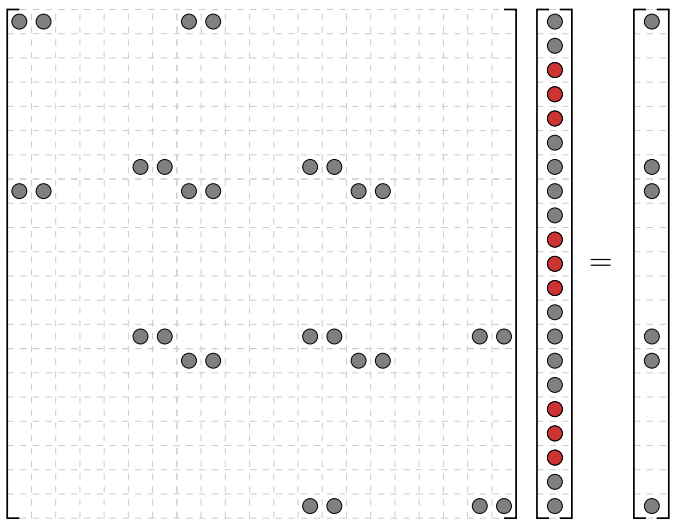
\includegraphics[scale=.75]{images/sparsity_larger}
\end{center}
\end{frame}



%///////////////////////////////////////////////////////////////////////
%////////////////////////// NUMERICAL RESULTS //////////////////////////
%///////////////////////////////////////////////////////////////////////





%////////////////////////// FFT //////////////////////////

\begin{frame}{Parallel FFT Solver Test Problem}
In the following numerical experiment $k$ is defined by 
\[k(z) = a - b\sin(cz)\]
 with $a > b \ge 0$. To test the accuracy, consider the analytic solution
\[u(\vec{x}) = \sin\l(\beta x\r) \sin\l(\gamma y\r)e^{-k(z)/c} \]
where $\beta^2+\gamma^2 = a^2 + b^2$. This gives the right-hand side
\[f(\vec{x}) = -b(2a+c)\sin(cz)e^{-k(z)/c}\sin(\beta x)\sin(\gamma y).\]
The domain under consideration is $\Omega = [0,\pi]\times [0,\pi] \times [0,\pi].$ 

\textbf{Turkel, D. Gordon, R. Gordon, and Tsynkov (2013)}
\textbf{}
\end{frame}

\begin{frame}{Parallel FFT Solver Accuracy}
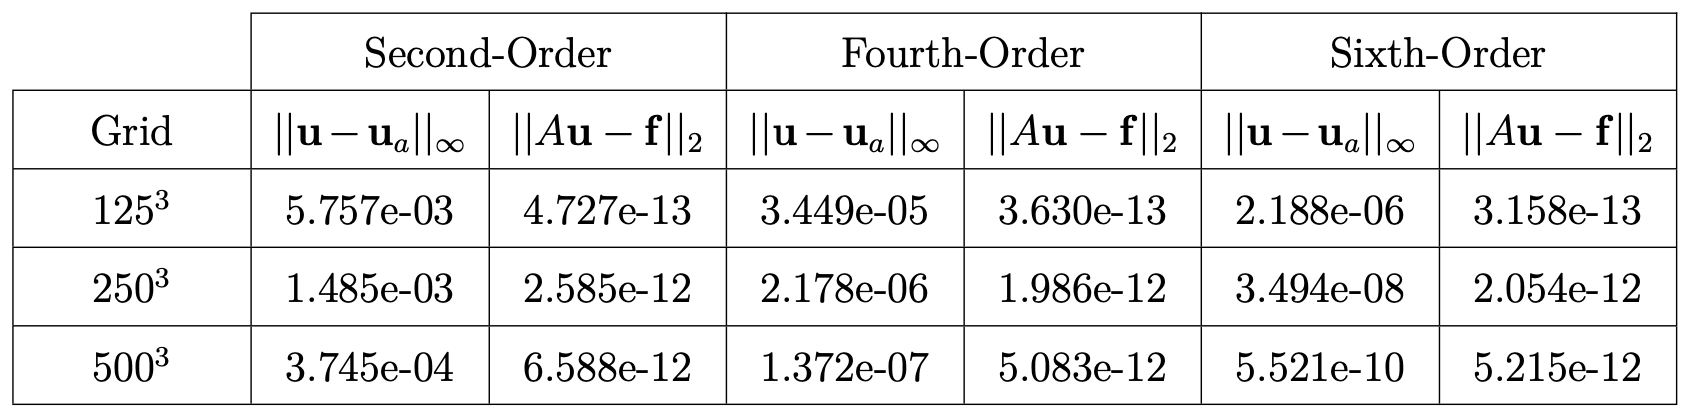
\includegraphics[scale=.395]{images/fft_convergence}
\end{frame}

\begin{frame}{Parallel FFT Solver OpenMP vs MPI on $512^3$}
\begin{center}
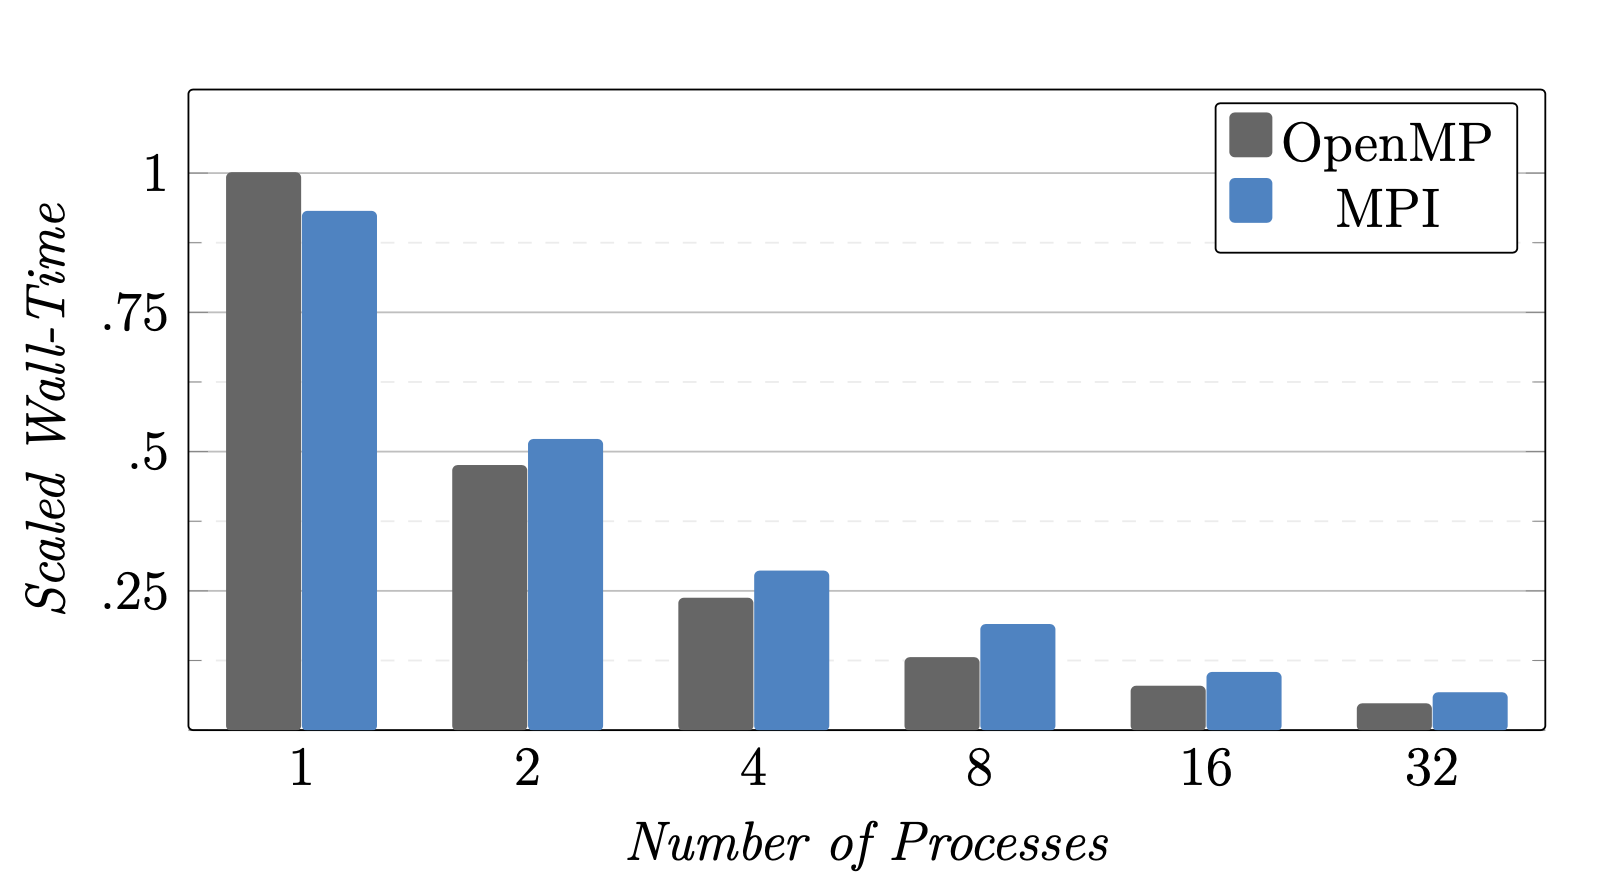
\includegraphics[scale=.35]{images/chart_var}
\end{center}
\end{frame}

\begin{frame}{Parallel FFT Solver Hybrid on $512^3$}
\begin{center}
\begin{tabularx}{\textwidth}{|X|X|X|X|X|X|X|}\hline
n\textbackslash t&1&2&4&8&16&32\\ \hline
1& 39.61&  21.73& 12.93& 8.83& 6.84& 5.62
\\ \hline
2& 19.87& 10.94& 6.48& 4.56& 3.48& 2.92
\\ \hline
4& 9.99& 5.66& 3.48& 2.52& 2.10& 1.82
\\ \hline
8& 5.27& 3.11& 1.99& 1.55& 1.37& 1.27
\\ \hline
16& 2.49& 1.42& 0.85& 0.64& 0.58& 0.58
\\ \hline
32& 1.85& 1.33& 1.09& 0.93& 0.76& 0.80
\\ \hline
\end{tabularx}
\end{center}
\end{frame}

\begin{frame}{Parallel FFT Solver Hybrid on Large Grids}
\begin{center}
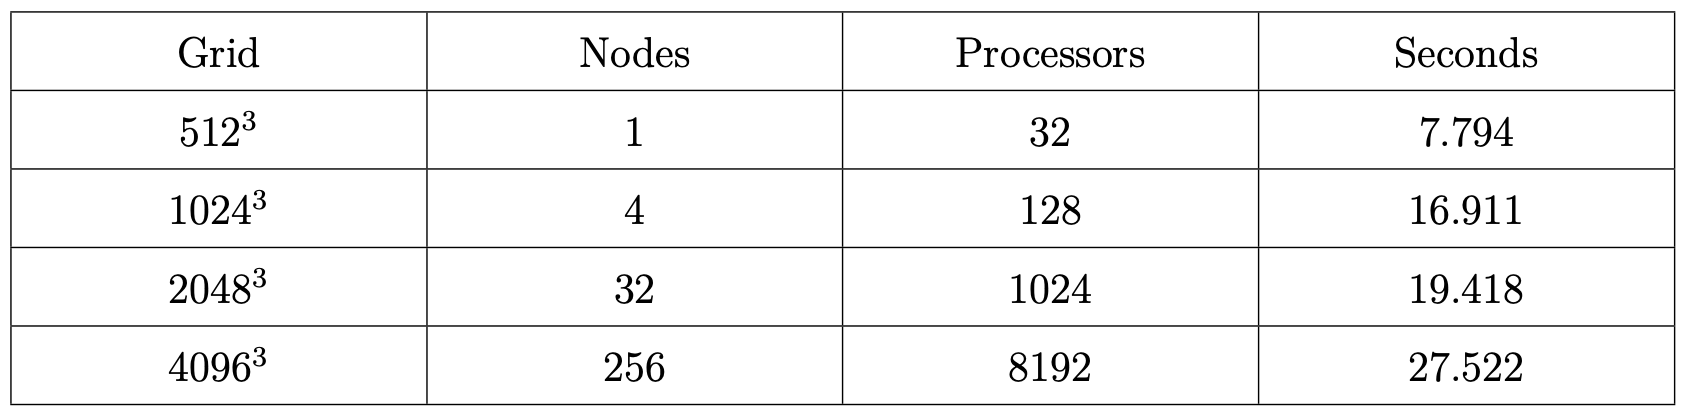
\includegraphics[scale=.4]{images/hyb_Large}
\end{center}
%For further detail on the FFT Solver see \cite{parallel_paper}.

\begin{itemize}
\item Turkel's iterative method required 267 minutes with 10000 iterations for a $402^3$ grid, roughly 65 million grid points.
\item The parallel FFT method solved a problem roughly 103 times larger and approximately 572 times faster.
\end{itemize}
\end{frame}


%////////////////////////// PFFT //////////////////////////


\begin{frame}{Parallel Partial FFT Solver Test Problem}
Two tests are considered here. First, let $k=\sqrt{439.2}$. Consider the function
\[\phi(x) = \exp\l(ik(x+1)\r) + \exp\l(-ik(x-1)\r) - 2. \]
In the two-dimensional case the analytic solution on the domain $\Omega = \l[-1,1\r]\times\l[-1,1\r]$ is given by $u(x,y) = \phi(x)\phi(y)$. The right-hand side follows
\[f(\vec{x}) = -k^2\l[\phi(x)\phi(y) - 2\phi(x) - 2\phi(y)\r].\]

\vtab
The next test assumes that $k = 2\pi$ on the domain $\Omega = [0,1]\times [0,1]$.
\end{frame}


\begin{frame}{Parallel Partial FFT Solver Accuracy}
\begin{center}
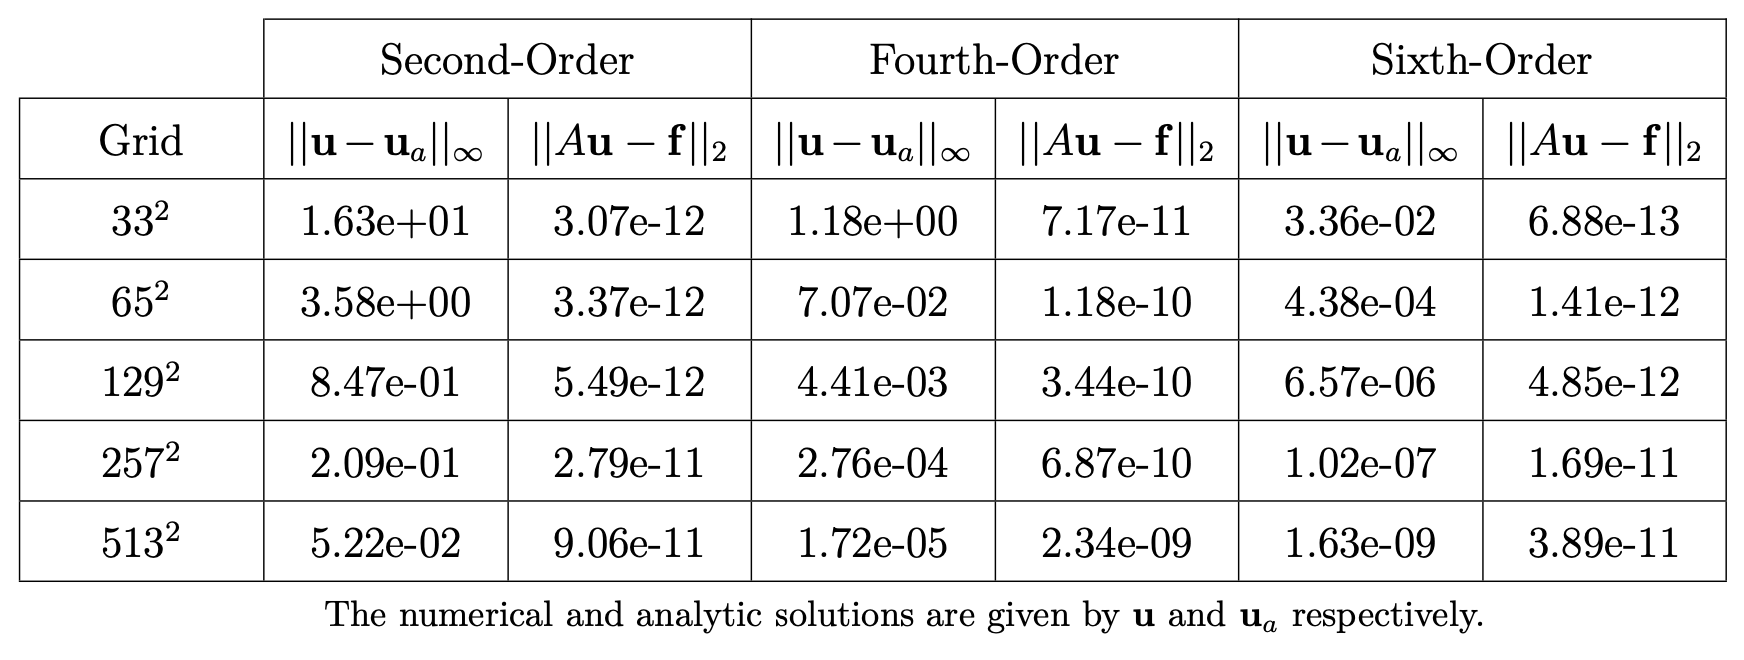
\includegraphics[scale=.395]{images/conv}
\end{center}
\end{frame}

\begin{frame}{Second Order Parallel Solver Comparison Uniform Grid}
\begin{center}
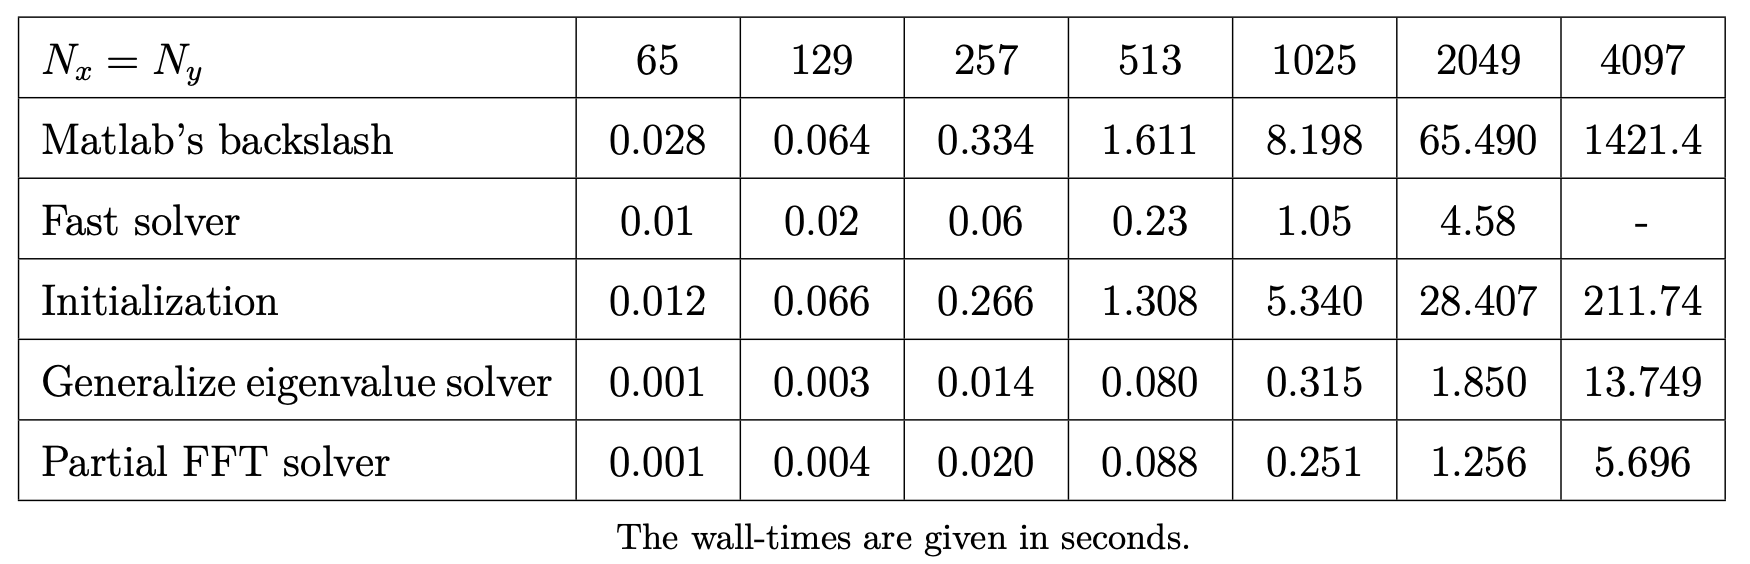
\includegraphics[scale=.395]{images/tv_uni}
\begin{itemize}
\item The ``fast solver" was developed by Toivanen and Wolfmayr (2020). 
\item The fast solver times come from a Matlab implementation.
\end{itemize}
\end{center}
\end{frame}

\begin{frame}{Second Order Parallel Solver Comparison Nonuniform Grid}
\begin{center}
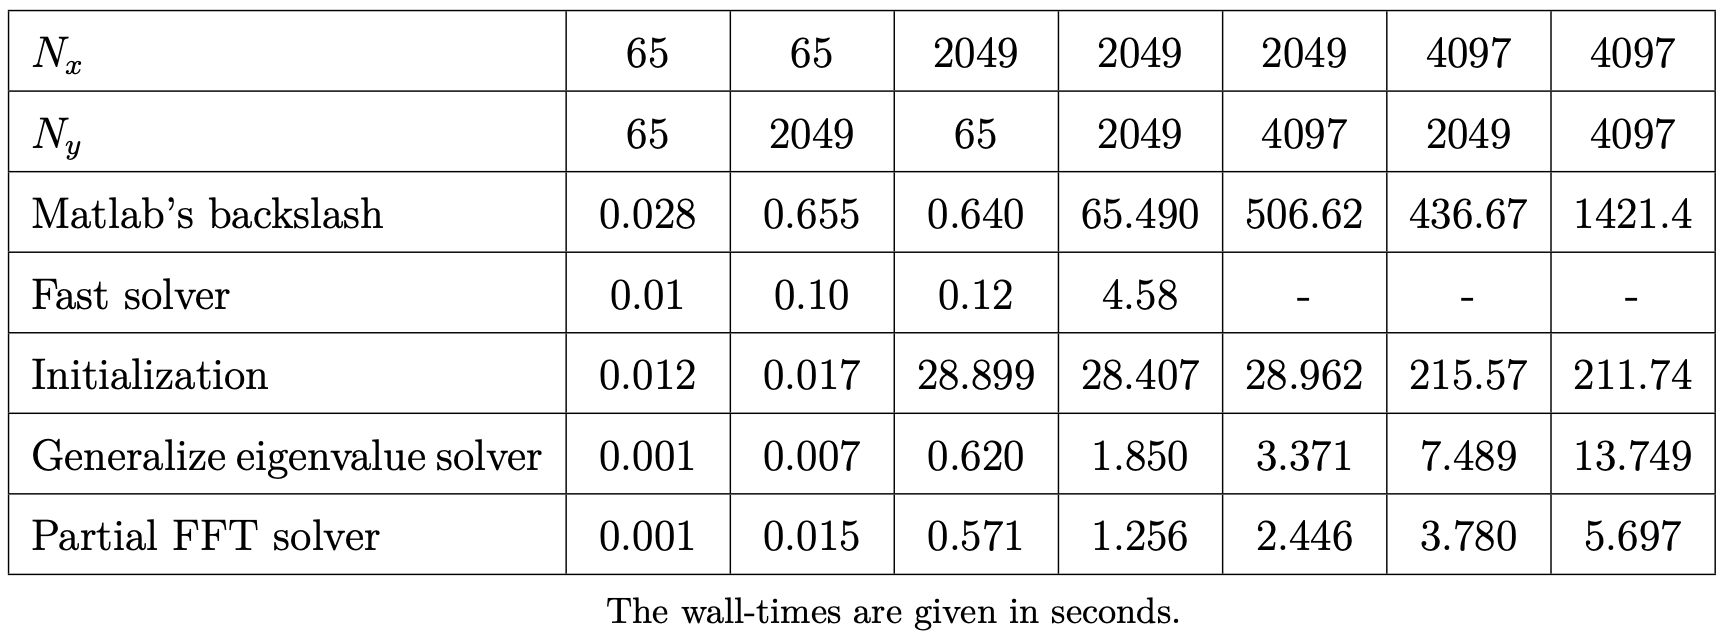
\includegraphics[scale=.395]{images/tv_nonuni}
\begin{itemize}
\item Faster solution with more grid points in the vertical direction due to parallelism.
\end{itemize}
\end{center}
\end{frame}


%\begin{frame}{Description of Variable Problem}
%\end{frame}


\begin{frame}{Parallel Partial FFT Solver Time Reduction OpenMP}
\begin{center}
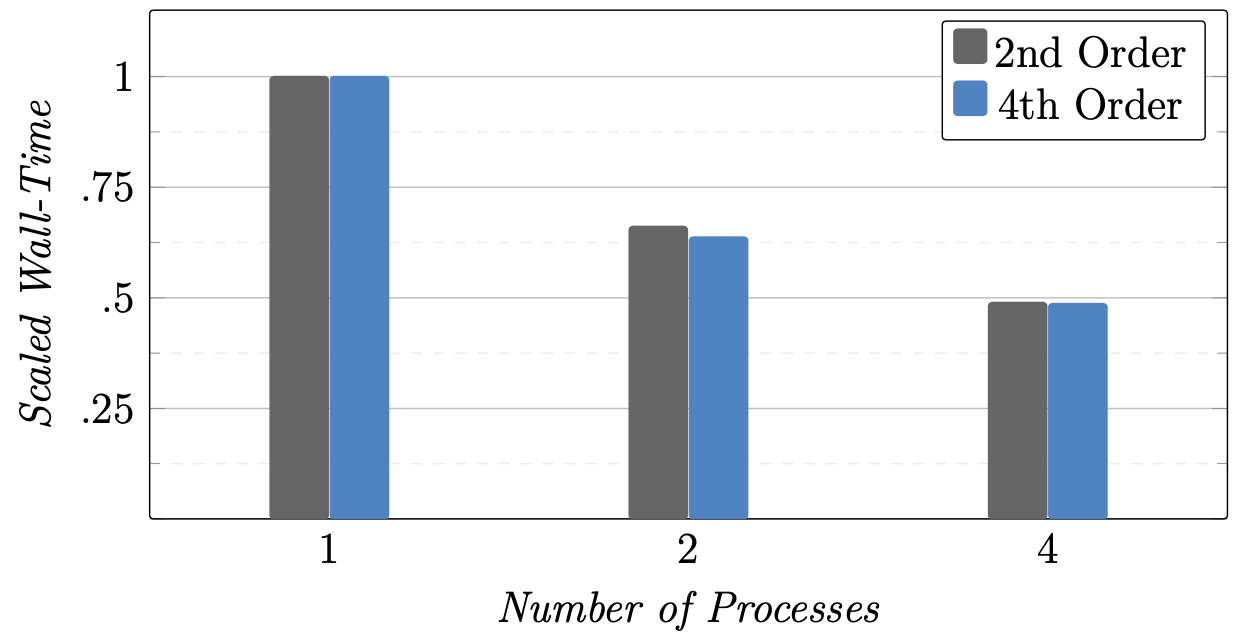
\includegraphics[scale=.45]{images/kz}\\
\begin{itemize}
\item Grid size of $4097^2$.
\item An extension to variable $k$, beyond the capability of the ``fast solver" by Toivanen and Wolfmayr (2020). 
\end{itemize}
\end{center}
\end{frame}





%////////////////////////// INCLUSION PROBLEM //////////////////////////


%\begin{frame}{Inclusion Test Problem}
%The domain considered is $\Omega = [-1,1]\times[-1,1]$. The function $k(\vec{x})$ is defined as
%\[k(\vec{x}) = \begin{cases}
%439.2 & \text{ if } y < 0\\
%1273+31i & \text{ if } y\ge 0 \text{ and }y\notin S \\
%1050+2.26i & \text{ if } y\in S
%\end{cases}\]
%where $S=\{\vec{x}\in\Omega\mid |x-.3|\le .15 \text{ and } |y-.2|<.04 \}$ is the set of grid points within the rectangular inclusion with width .15, height .04 and center (.03,.2). The right-hand side is given by
%\[f(\vec{x})=
%\begin{cases}
%0, &\text{ outside inclusions,}\\
%%(k_g^2-k^2(\vec{x}))u_0(\vec{x}), &\text{ inside inclusions}
%g(\vec{x}), &\text{ inside inclusions}
%\end{cases}\]
%where $g(\vec{x})$ is a function representing the wave produced by ground penetrating radar.
%\end{frame}

\begin{frame}{Inclusion Test Problem}
The function $k(\vec{x})$ is defined as
\[k(\vec{x}) = \begin{cases}
439.2 & \text{ if } y < 0\\
1273+31i & \text{ if } y\ge 0 \text{ and }y\notin S \\
1050+2.26i & \text{ if } y\in S
\end{cases}\]
where $S=\{\vec{x}\in\Omega\mid |x-.3|\le .15 \text{ and } |y-.2|<.04 \}$ is the set of points within the rectangular inclusion with width .15, height .04 and center (.03,.2). The air and soil interface is at $y=0$.
\end{frame}

\begin{frame}{Inclusion Test Problem Continued}
The domain considered is $\Omega = [-1,1]\times[-1,1]$ and right-hand side given by
\[f(\vec{x})=
\begin{cases}
0, &\text{ outside inclusions,}\\
%(k_g^2-k^2(\vec{x}))u_0(\vec{x}), &\text{ inside inclusions}
g(\vec{x}), &\text{ inside inclusions}
\end{cases}\]
where $g(\vec{x})$ is a function corresponding to the electromagnetic signal produced by ground penetrating radar.
\end{frame}

%\begin{frame}{Accuracy of Inclusion Solution Calculated in Parallel}
%\begin{center}
%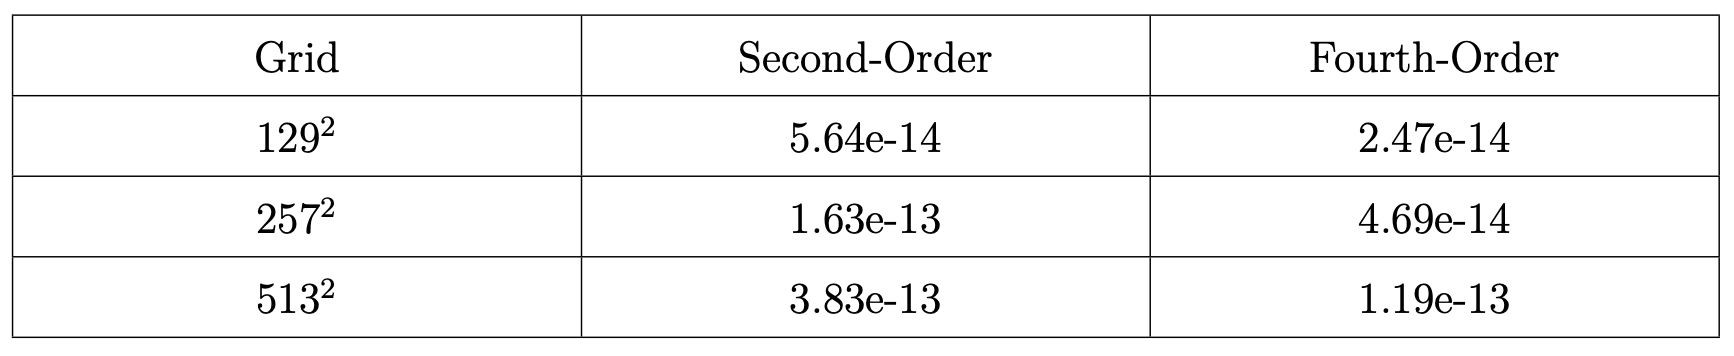
\includegraphics[scale=.37]{images/inc_acc}
%\end{center}
%\end{frame}

\begin{frame}{Subsurface Inclusion Accuracy and Parallel Time Reduction}
\begin{center}
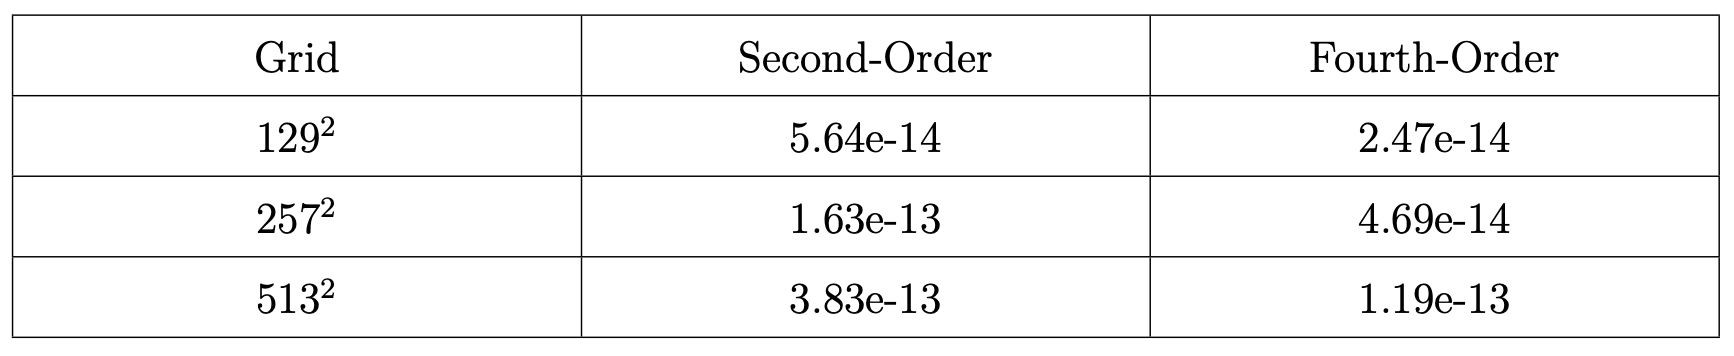
\includegraphics[scale=.35]{images/inc_acc}\\
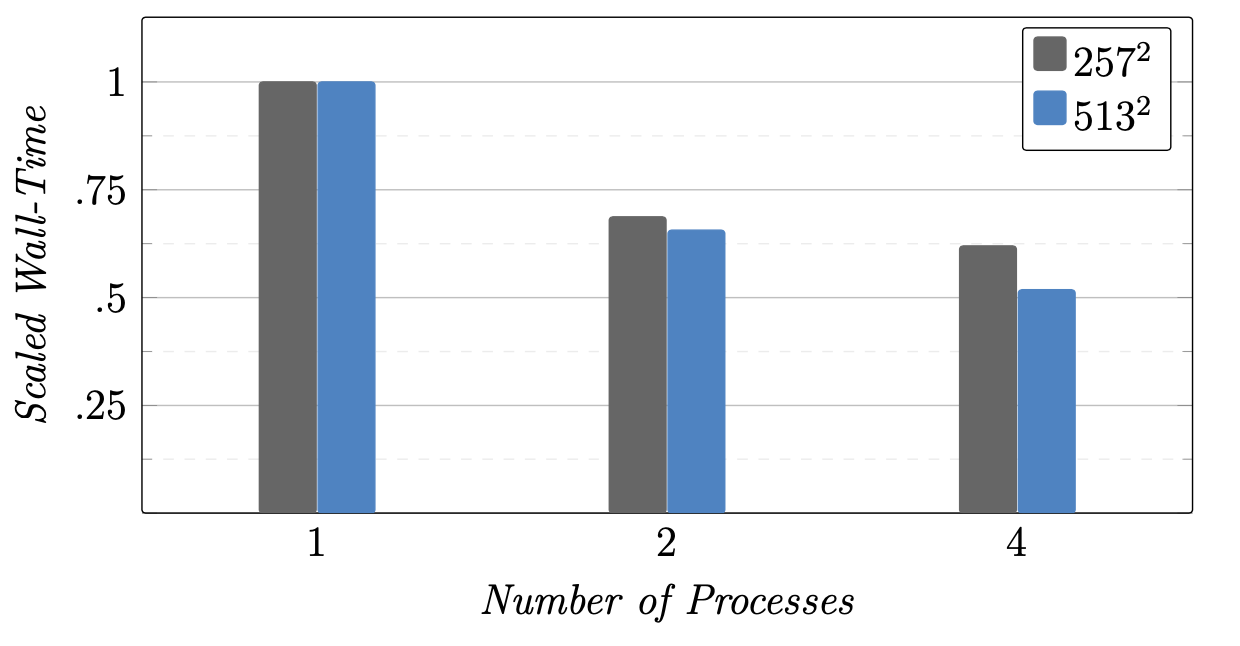
\includegraphics[scale=.45]{images/inc_scale}
\end{center}
\end{frame}

\begin{frame}{Subsurface Inclusion and Solution Image}
\begin{center}
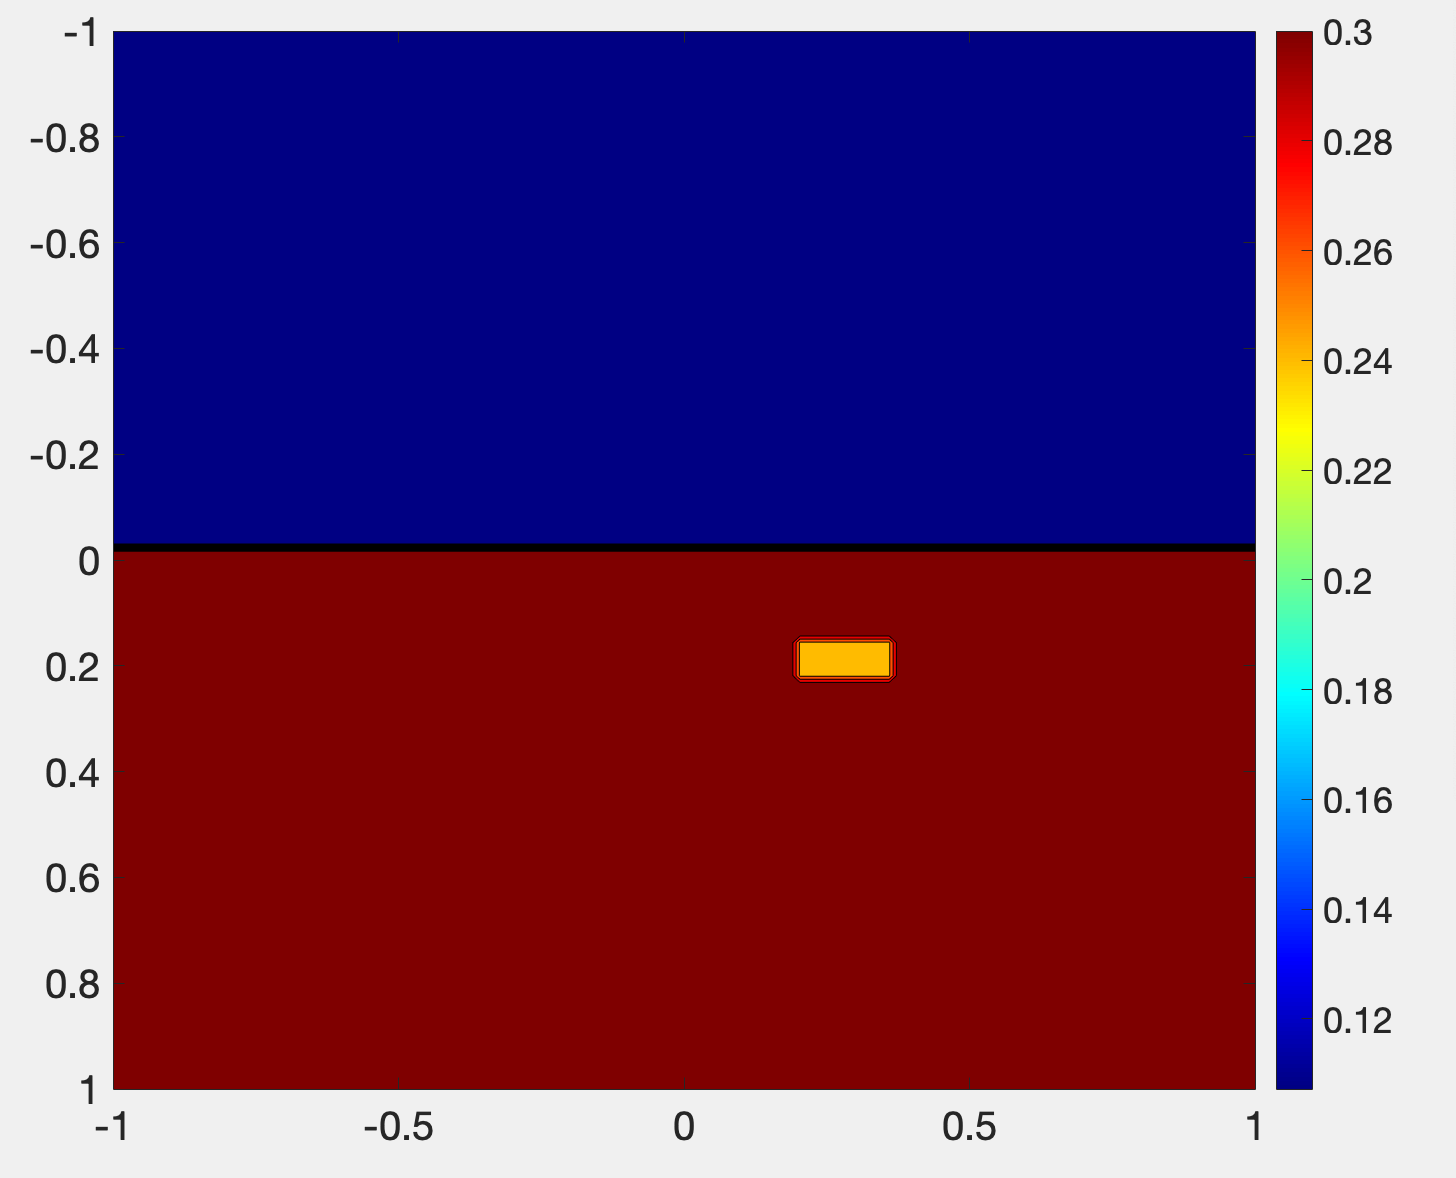
\includegraphics[scale=.2252]{images/bg}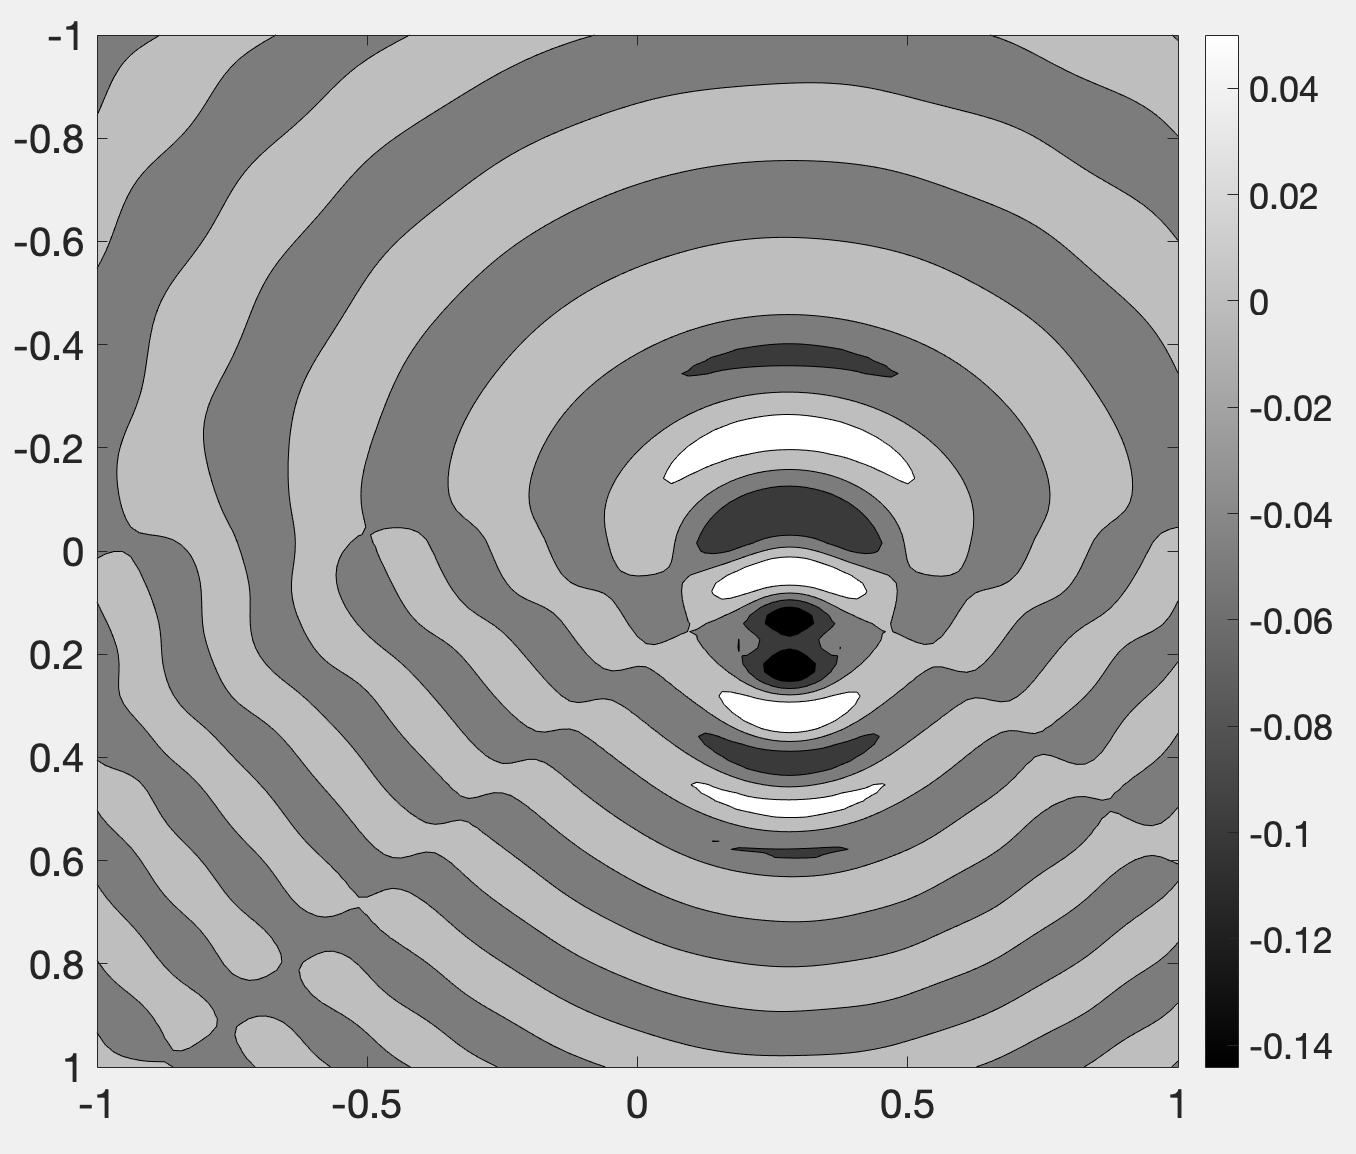
\includegraphics[scale=.23]{images/sol}
\end{center}
\end{frame}







%////////////////////////// CONCLUSION //////////////////////////

\begin{frame}{Conclusion}
\begin{itemize}
\item Presented a novel direct parallel partial FFT-type algorithm for the numerical solutions of the two- and three-dimensional Helmholtz equations.\\[1em]
\item Governing equations were discretized by high-order compact finite-difference schemes.\\[1em]
\item Presented numerical results demonstrating the accuracy and scalability of the direct parallel method.\\[1em]
\end{itemize}
\end{frame}

%\begin{frame}{Future Work}
%%	Add slide on applications ie the questions they asked
%%  		- non uniform domain and angled plane wave
%\begin{itemize}
%\item Potential performance improvements
%\begin{itemize}
%\item Reduced memory usage
%\item SuperLU solver vs LAPACK\\[1em]
%\end{itemize}
%\item Preconditioner for GMRES solver
%\begin{itemize}
%%\item Angled source wave
%\item Non-uniform subsurface domain\\[1em]
%\end{itemize}
%\item Comparison between direct DST and DST via FFT\\[1em]
%\item Solutions used to produce a training set for neural network 
%\end{itemize}
%\end{frame}

\begin{frame}{Thank you}
\begin{itemize}
\item Family and friends\\[1em]
\item Yury Gryazin,  Ph.D.\\[1em]
\item Yun Teck Lee, M.S.\\[1em]
\item Idaho State University Department of Mathematics and Statistics\\[1em]
\end{itemize}
\end{frame}





\begin{frame}{References}
\begin{thebibliography}{9}
\bibitem{lele}
{Sanjiva Lele.}
\textit{Compact finite difference schemes with spectral-like resolution.}
{Journal of Computational Physics 103 (1992) 16-42.}\\

\bibitem{Nabavi}
{Majid Nabavi, M.H. Kamran Siddiqui, and Javad Dargahi.}
\textit{A new 9-point sixth-order accurate compact finite-difference method for the Helmholtz equation.}
{Journal of Sound and Vibration 307 (2007) 972-982.}\\

\bibitem{Sutmann}
{Godehard Sutmann.}
\textit{Compact finite difference schemes of sixth order for the Helmholtz equation.} 
{Journal of Computational and Applied Mathematics 203 (2007) 15-31.}\\

\bibitem{turkel}
{Eli Turkel,  Dan Gordon,  Rachel Gordon, and Semyon Tsynkov.}
\textit{Compact 2D and 3D Sixth Order Schemes for the Helmholtz Equation with Variable Wave Number.}
{Journal of Computational Physics 232 (2013) 272-287.}\\
\end{thebibliography}
\end{frame}

\begin{frame}
\begin{thebibliography}{9}


\bibitem{Elman}
{Howard Elman and Dianne O'Leary}
\textit{Efficient iterative solution of the three-dimensional Helmholtz equation.}
{Journal of Computational Physics 142 (1998) 163-181.}\\


\bibitem{dg1}
{Yury Gryazin, Michael Klibanov, and Thomas Lucas.}
\textit{GMRES Computation of High Frequency Electrical Field Propagation in Land Mine Detection.}
{Journal of Computational Physics 158 (2000) 98-115.}\\

\bibitem{spie19}
{Yun Teck Lee,  Yury Gryazin, and Ronald Gonzales.}
\textit{Scalable high-resolution algorithms for land-mine imaging problem.}
{SPIE Proceedings 11012 (2019) 241-250.}\\

\bibitem{parallel_paper}
{Ronald Gonzales,  Yury Gryazin, and Yun Teck Lee.}
\textit{Parallel FFT algorithms for high-order approximations on three-dimensional compact stencils.}
{Parallel Computing 103 (2021) 102757.}\\

\end{thebibliography}
\end{frame}


\begin{frame}
\begin{thebibliography}{9}




\bibitem{toivanen}
{Jari Toivanen and Monika Wolfmayr.}
\textit{A fast Fourier transform based direct solver for the Helmholtz problem.}
{Numerical Linear Algebra with Applications, arXiv:1809.03808 (2020).}\\


\bibitem{spie22}
{Ronald Gonzales and Yury Gryazin.}
\textit{Parallel High-Resolution Compact Partial FFT-Type Direct Algorithms for Subsurface Scattering Problems.}
{SPIE Proceedings (2022)}


\end{thebibliography}
\end{frame}








 
\end{document}